\chapter{Sticky and slippery soft obstacles}\label{ch02_soft}

The diffusion of macromolecules in crowded environments is generally slowed
relative to the uncrowded case, and particles can undergo transient
anomalous subdiffusive motion~\cite{hofling_anomalous_13}.  The motion of lipids or
macromolecules within biological membranes can be affected by
crowding~\cite{schutz_singlemolecule_97,schutz_properties_00,
  nicolau_sources_07, weigel_ergodic_11, javanainen_anomalous_13,
  krapf_mechanisms_15, jeon_protein_16, sadegh_plasma_17} because the membrane
contains both macromolecules and inhomogeneities in membrane
composition~\cite{petropoulos_membrane_90, veatch_organization_02}. In the cell
interior, macromolecules, organelles and other cellular structures can inhibit
motion, or in contrast, enhance sampling of non-crowded
regions~\cite{stylianidou_cytoplasmic_14}.  Biological crowders can also contain
interaction sites which further modify the macromolecular
motion~\cite{crowley_protein_11}.  The kinetics and equilibrium behavior of
interactions between mobile proteins can be modified by
crowding~\cite{mourao_connecting_14, zhdanov_kinetics_15}. The magnitude of the
effects of crowding on macromolecular motion and reactions is important to
determine the limiting rate of biological processes such as signaling receptor
activation.
 
Although most theoretical work has focused on anomalous diffusion in crowded
systems made up of impenetrable obstacles with attractive or repulsive
surfaces~\cite{saxton_lateral_87, saxton_anomalous_94, saxton_anomalous_96,
  ellery_characterizing_14, ellery_analytical_16}, there is growing evidence of
the importance of soft compartments and barriers in biological systems.  In
membranes, lipids may be only partially excluded from lipid rafts or domains.
When they do interact, they can still diffuse within
them~\cite{fujiwara_phospholipids_02, forstner_attractive_08,
  ehrig_nearcritical_11, silvius_partitioning_05}.  Lipid motion can be
hindered, though not stopped, near $\alpha$-synuclein protein
aggregates~\cite{iyer_membranebound_16}. For all of these cases, theoretical
considerations of a two-dimensional system should include the effects of soft
interaction potentials and bound-state mobility.

Inside the cell, intrinsically disordered or low-complexity domains can act as
soft obstacles or wells, with rapid diffusion within the wells.  Membraneless
organelles spontaneously form from low-complexity domain proteins. They are
typically highly dynamic assemblies~\cite{brangwynne_germline_09}, which show
fast intra-particle diffusion times, and allow rapid entry and exit of
constituents~\cite{molliex_phase_15}.  Proteins that interact with
intrinsically disordered proteins can still diffuse during the binding
interaction~\cite{hough_molecular_15, raveh_slideandexchange_16}.  This effect
may be particularly pronounced in the central channel of the nuclear pore
complex, which contains a high density of binding sites on intrinsically
disordered domains.  Recent simulation work suggests that the disordered protein
binding pockets can exchange on transport
factors~\cite{raveh_slideandexchange_16}, providing a clear mechanism for
mobility while bound to an obstacle.  Particles are weakly excluded from
individual disordered protein chains due to the lowering of the polymer chain
entropy~\cite{timney_simple_16}, but are expected to allow other macromolecules
to enter, and pass through, the space that they occupy.  The increasingly
recognized importance of proteins that are intrinsically disordered or contain
low-complexity domains (within their assemblies) warrants a more careful
consideration of the differences between the previously well-studied models, in
which binding immobilizes the bound species, and a model that includes soft
interactions and obstacles or barriers in which the bound species may remain
mobile.

Motivated by the biological importance of binding interactions which can retain
mobility of the bound particle, we studied a minimal model with bound tracer
mobility \figrefp{fig:soft_model}. In our model, tracer particles move on a 2D
or 3D lattice in the presence of immobile obstacles, to which the tracers can
bind.  A primary distinction between our model and many others that consider
binding or adhesion is that others typically consider adhesion between a tracer
and an adjacent hard obstacle in which there is no overlap between tracers and
a hard obstacle's core~\cite{saxton_anomalous_96, wedemeier_how_09,
  ellery_analytical_16}.  Here, obstacles are soft: tracer particles can overlap
with obstacles, with an energy penalty (or gain) $\Delta G$ upon moving to a
lattice site occupied by an obstacle. Unlike previous work modeling lipid rafts,
we closely examine the dependence on binding, instead of just pure exclusion or
free entry into lipid regions~\cite{nicolau_sources_07}.

To understand the effects of bound mobility, we first consider the limits of
`sticky obstacles', in which tracers are immobile while bound, and `slippery
obstacles', in which tracers are mobile while bound.  We use lattice Monte Carlo
methods to explore a range of binding energies and obstacle filling fractions.  We
also examine the effects of semi-sticky obstacles, \textit{i.e.,} intermediate
bound diffusion coefficients, and obstacle size effects. Our work demonstrates
how diffusion is altered in a crowded environment comprised of compartments with
different properties, such as a cell~\cite{berry_monte_02}.  Our results
demonstrate how binding and bound-state motion independently impact particle
dynamics, including long-time normal diffusion and anomalous diffusion.  Bound
tracer mobility increases the long-time diffusion coefficient, reduces the
transient anomalous time, and eliminates caging for all times typically observed
above the percolation threshold. These results demonstrate that mobility of
bound particles can benefit biological systems by allowing mobility even in
highly crowded environments.

\section{Anomalous diffusion}
Fractional  or anomalous diffusion has been experimentally measured in cells,
using fluorescence recovery after photobleaching~\cite{feder_constrained_96},
fluorescence correlation spectroscopy~\cite{weiss_anomalous_04,
  banks_anomalous_05}, and single-particle tracking~\cite{ghosh_automated_94}.
Anomalous diffusion in crowed environments is typically described by a MSD that
is no longer linear in time~\cite{metzler_random_00}
%
\begin{equation}
  \label{eqn:msd_anom}
  \langle r ^ 2 \rangle \sim t ^ {\alpha},
\end{equation}
%
where $\alpha$ is called the anomalous coefficient. The magnitude of $\alpha$
describes the type of diffusion: subdiffusive ($\alpha < 1$), Fickian
($\alpha=1$), and superdiffusive ($\alpha > 1)$. There is a fractional diffusion
equation associated with the dynamics in \eqnref{eqn:msd_anom}, but we will
neglect discussing it further (see~\cite{metzler_random_00,
  sokolov_fractional_02} for more details).
  
In a traditional Fickian random walk, steps occur at a fixed interval.  In a
continuous-time random walk, this assumption is relaxed. The waiting-time before
taking a step is sampled from a distribution. A continuous-time random walk in
which the mean waiting time diverges, \textit{e.g.}, with a power law
waiting-time distribution, results in anomalous
diffusion~\cite{metzler_random_00, sokolov_fractional_02}. 

An inhomogeneous random arrangement of hard obstacles can provide an irregular
step rate that introduces memory~\cite{sokolov_fractional_02}.  One way of
viewing viewing anomalous diffusion of a tracer in the presence of obstacles is
by considering the fractal structure of an obstacle
cluster~\cite{saxton_lateral_87,saxton_anomalous_94}.  Clusters of random hard
objects are fractal over short length scales and homogeneous over larger length
scales.  On length scales larger than the fractal structure, for which the
landscape is homogeneous, the diffusion becomes normal ($\alpha=1$).  The
Fickian diffusion constant is a measure of the long time behavior of a tracer
diffusing in this homogeneous environment. When $\alpha \neq 1$, a tracer is
exploring length scales in which clusters of hard obstacles are
fractal~\cite{saxton_lateral_87}. 

The anomalous coefficient characterizes the non-homogeneity and fractal
structure of a local landscape.  It does not describe the time it takes to
escape an trapping cage; just that there is a possibility that the landscape
could trap a tracer.  In the $\alpha \rightarrow 0$ limit, a tracer is fully
caged.  

\section{Lattice models}

Lattice Monte Carlo is a valuable tool for studying diffusion in crowed media. A
tracer particle undergoes a random walk on a lattice. Obstacles on the lattice
can alter dynamics of the tracer by inhibiting steps, lowering the step attempt
rate, etc.  The typical procedure is that a random number is generated at a
given time step.  Based on that number, a particle will attempt a step in a
given direction. If there are obstacles present, a move will be accepted or
rejected based on the interaction with that obstacle. For example, if an
obstacle is impenetrable and a tracer tries to step there, the move is rejected.
We can also imagine obstacles affecting the local energy landscape. If there is
an energy difference $ \Delta E$ associated with moving between lattice sites,
moves are accepted with a probability based on the Boltzmann factor
$P_{\text{accept}} \sim e^{-\beta \Delta E } $ where $\beta =  1 / k_B T$.

Our model seeks to build on stochastic lattice-gas models that have been
important to understanding tracer dynamics in the presence of immobile and
mobile hard obstacles~\cite{saxton_lateral_87}, anomalous
subdiffusion~\cite{saxton_anomalous_94}, and effects of binding on
diffusion~\cite{saxton_anomalous_96}. Saxton showed that the tracer diffusion
coefficient drops to zero at the percolation threshold, the critical
concentration of obstacles at which a continuous path of vacancies (through which
a tracer can move) no longer exists. Above this percolation threshold, diffusion
is anomalous at long times.  The effects of tracer and obstacle
size~\cite{ellery_characterizing_14,ellery_calculating_15,ellery_modeling_16}
and adhesion and repulsion to sites adjacent to
obstacles~\cite{ellery_analytical_16} on transient subdiffusion and long-time
diffusion have been studied. Extensions to mobile obstacles that interact with
each other have demonstrated how obstacle clustering dynamics can influence the
diffusivity of tracers~\cite{nandigrami_gradientdriven_17}. 

Numerically exact methods for calculating diffusion coefficients using the
Nernst-Einstein relation~\cite{mercier_numerically_99, mercier_numerically_99a}
and Markov chains~\cite{ellery_communication_16} have been implemented as a
different approach to analyzing these systems; the Nernst-Einstein approach can
lower the computational cost of measuring diffusion coefficients for lattice
gases~\cite{ellery_calculating_15}.  Protein motion in polymer networks has been
studied using random walk and self-avoiding-chain models for
immobile~\cite{wedemeier_modeling_07} and mobile~\cite{wedemeier_how_09,
  wedemeier_anomalous_09} hard chains. Studies of chains with binding sites
found that modeling chain dynamics allowed a mapping onto randomly distributed
obstacles with an effective volume, and showed how sliding along a defined chain
can effect tracer dynamics~\cite{wedemeier_role_08, wedemeier_anomalous_09}.
Note, this mapping, which amounts to a mean-field approximation of obstacles, is
not valid in the limit of static obstacles. In some previous work, the effects
of binding and sliding while bound were entangled because both effects were
encoded by a single parameter~\cite{wedemeier_role_08, wedemeier_anomalous_09}.
Domains with different diffusion coefficients and sizes (to model lipid rafts)
have been studied, but the analysis only included total or no exclusion although
it was noted that binding effects could play a large
role~\cite{nicolau_sources_07}.

\section{Model}
% figure01 %
%\begin{figure}[htbp]
\begin{figure}[!ht]
  \begin{center}
    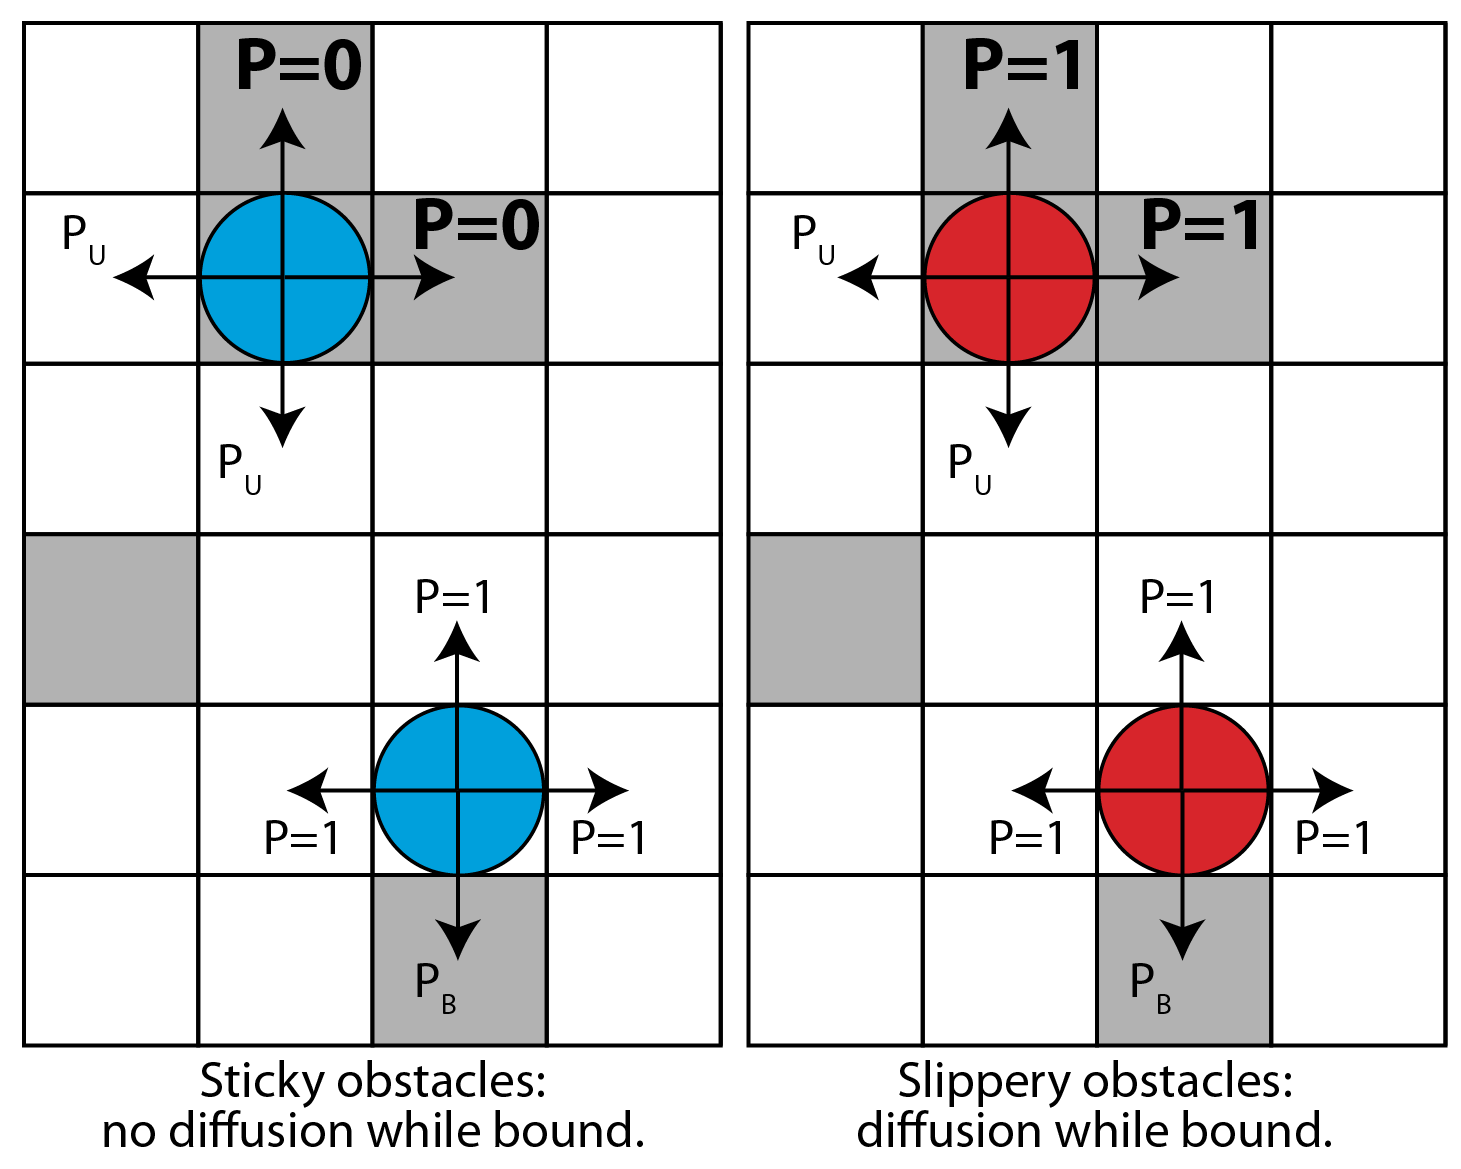
\includegraphics[width=100mm]{figs/ch02_soft/soft_model.png}
  \end{center}
	\caption[Soft sticky and slippery model schematic]
    {Model schematic. Tracers (colored circles) hop on a lattice
    of empty sites (white squares) and obstacles (gray
    squares). Tracer binding with a soft interaction potential allows
    them to overlap with obstacles (top). For sticky obstacles, the
    only allowed moves of a bound tracer are to empty sites
    (unbinding).  For slippery obstacles, tracers can hop to other
    obstacles while remaining bound.  Arrows denote possible moves and
    P the probability that a given move is accepted.}\label{fig:soft_model}
\end{figure}

In our model, tracer particles undergo a random walk on a square lattice and
interact with immobile obstacles. The interaction is characterized by a binding
free energy; for simplicity, we neglect any additional activation barrier.  The
characteristic binding free energy change of a tracer that hops from an empty
site to an obstacle site is $ \Delta G $ (in units where $k_B T = 1$).  We
consider both attractive ($ \Delta G < 0 $) and repulsive ($ \Delta G > 0 $)
obstacles. We use the Metropolis algorithm~\cite{metropolis_equation_53} to
accept or reject candidate binding (probability $P_B$) and unbinding
(probability $P_U$) events. Each tracer occupies a single site lattice site, but
the obstacle size is varied to represent domains of characteristic size.
Obstacles are squares with sides of length $l_{\rm obst}$, measured in units of
the lattice spacing.
 
To study the effects of tracer particle motion while bound, we considered the
limits of perfectly sticky and slippery obstacles \figref{fig:soft_model}, as
well as the intermediate `semi-slippery' case. In all models, obstacles are
soft, so that tracers overlap with obstacles when bound. For sticky obstacles,
no hopping between obstacle sites can occur, but tracers can exit an obstacle to
an unoccupied site.  For slippery obstacles, tracers can hop between adjoining
obstacles while remaining bound.  In the limit of perfectly slippery obstacles,
bound motion is identical to unbound motion: there is no difference in hopping
rates between free and bound tracers. For semi-slippery obstacles, we vary the
bound diffusion coefficient.

\subsection{Simulation methods}

In our kinetic Monte Carlo scheme, at each time step a tracer attempts a move in
a randomly chosen direction. Moves from $ \mathbf {empty} \rightarrow \mathbf
{empty} $ are always accepted, $ \mathbf {empty} \rightarrow \mathbf {obstacle}$
moves are accepted with probability $ P_B = \mathbf {\min}( e^{-\Delta G}, 1) $,
$ \mathbf {obstacle} \rightarrow \mathbf {empty} $ moves are accepted with
probability $ P_U = \mathbf {\min}( e^{\Delta G}, 1 ) $, and $ \mathbf
{obstacle} \rightarrow \mathbf {obstacle} $ moves are always accepted/rejected
if obstacles are slippery/sticky \figrefp{fig:soft_model}; for semi-slippery
obstacles, the acceptance probability is $D_{\rm bound}/D_{\rm free}$. If a
tracer's move is rejected, it remains immobile for that time step. We assume
noninteracting tracers.

Initially, obstacles were uniformly randomly placed on the lattice, at the
specified filling fraction, without overlaps. Next, tracers were randomly placed
on obstacles and empty sites at their equilibrium occupancy, as determined by
the filling fraction of obstacles $\nu$, and binding energy $\Delta G$.  The
fraction of tracers on obstacles is proportional to the obstacle filling
fraction times the Boltzmann factor $\nu e^{-\Delta G}$, while the fraction of
tracers on empty sites is proportional to the fraction of empty sites $(1-\nu)$.
The equilibrium fraction of tracers on obstacles of size one is then
%
\begin{equation}
  \mathit{f}_{o} = 
    \frac{\nu e^{-\Delta G}}{\nu e^{-\Delta G} + \left(1 - \nu \right)}.
\end{equation}
%
Using an initial fraction of tracers bound to obstacles determined from $f_o$
avoids the time required for binding equilibration in the simulations, ensuring
that mean-squared displacement measurements are independent of time origin.

We performed 2D simulations with $ 200 $ tracers on a $ 256 \times 256 $
periodic lattice for $ 10^{5} - 10^{7.5} $ time steps, with a recording interval
of $ 10 - 100 $ steps. For each parameter set (determined by filling fraction
and binding energy), we averaged over $ 96 $ separate obstacle configurations.
We varied $\nu$ from 0 to 1 and $\Delta G$ from $-5$ to $10$. Three dimensional
simulations used similar parameters with a $ 256 \times 256 \times 256$ periodic
lattice. In the semi-slippery case, we varied the ratio of bound to free
diffusion coefficient $D_{\rm bound}/D_{\rm free}$ between 0 (perfectly sticky)
and 1 (perfectly slippery) in steps of 0.2, for binding energy $\Delta G = 1, 2,
3, \infty$ and for filling fraction, $ \nu = 0.3 $ and $ 0.6 $.  When varying
obstacle size, we used square obstacles with the length of a side, $l_{\rm
  obst}$, equal to odd values from 1 to 15. When varying obstacle size, we
studied repulsive obstacles, to understand how binding affects diffusion for
finite repulsion between the previously-studied free binding and pure exclusion
limit~\cite{nicolau_sources_07, ellery_characterizing_14}.

% figure 02 %
\begin{figure}[!hb]
  \begin{center}
    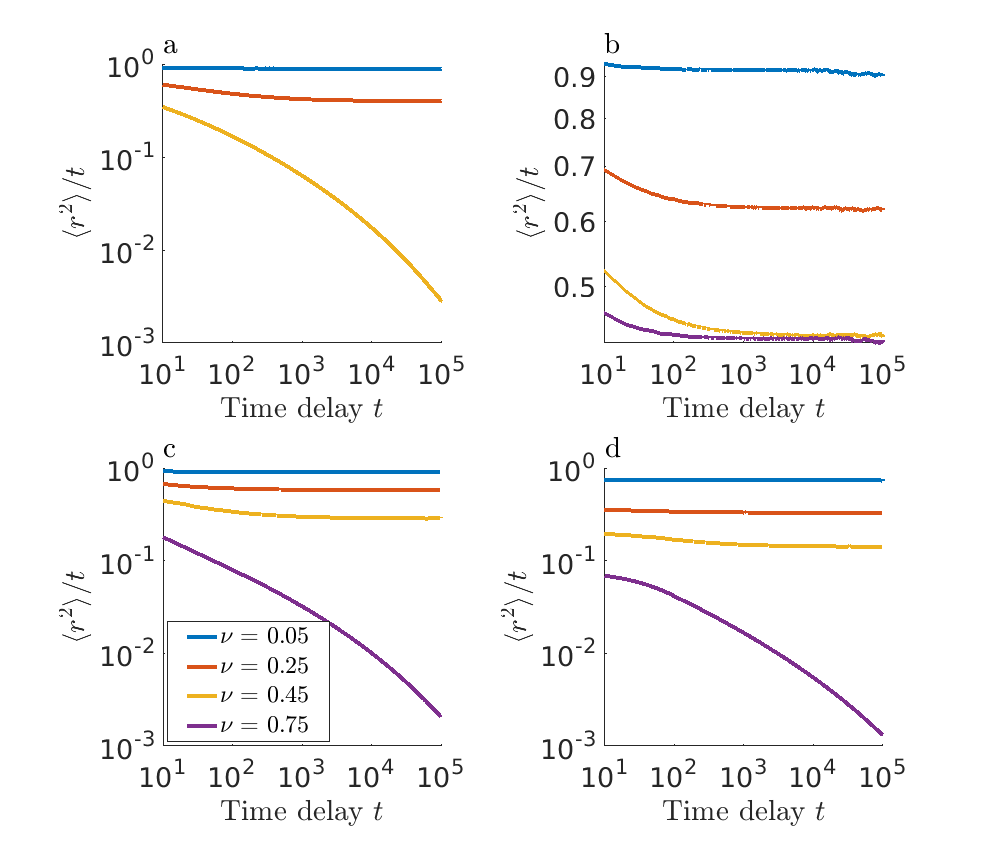
\includegraphics[width=150mm]{figs/ch02_soft/soft_msd_curves.png}
  \end{center}
  \caption[MSD curves]
	  {Mean-squared displacement $\langle r^2 \rangle$ divided by
    time delay $t$ as a function of time delay $ t $ for (a) impenetrable
    obstacles, (b) repulsive slippery obstacles ($ \Delta G = 2 $),
    (c) repulsive sticky obstacles ($ \Delta G = 2 $), and (d)
    attractive sticky obstacles ($ \Delta G = -2 $). Different colors
    correspond to different filling fraction $\nu$. Curves with
    non-zero slope indicate anomalous diffusion, and the horizontal
    asymptote indicates the long-time diffusion coefficient. Each
    curve represents an average over tracers, independent time
    windows, and obstacle configurations.}\label{fig:msd_curves}
\end{figure}


\subsection{Trajectory analysis}

We determined tracer mean-squared displacement (MSD) as a function of time delay
by averaging over all tracers, $ 100 $ randomly selected independent time
origins, and obstacle configurations. For long time delays for which $100$
independent time intervals were not available, we averaged over the maximum
number of independent time intervals. As previously mentioned, averaging over
time windows improves our statistics; note that the time origins are not unique,
since the placement of tracers in their equilibrium binding distribution ensures
that there is no initial binding equilibration time.  We have verified that
there are no aging effects~\cite{magdziarz_fractional_09, schulz_aging_14},
\textit{i.e.}, MSD measurements that depend on simulation time, in our model
(data not shown).
 
We sought to quantify the effects of binding and obstacle filling fraction on
tracer mobility.  In systems with either purely Fickian diffusion or particular
obstacle geometry, the mean-squared displacement grows as a power law in time:
%
\begin{equation}
  \label{eqn:msd_anom_full}
  \langle r^2 \rangle =  2dD t ^ {\alpha},
\end{equation}
%
where $\langle r^2 \rangle$ is the ensemble-, time-origin-, and
obstacle-configuration-averaged mean-squared displacement, $d$ the spatial
dimension, $D$ the diffusion coefficient, $\alpha$ the diffusion scaling
exponent, and $t$ the time delay. This fractional diffusion equation has been
studied extensively~\cite{metzler_random_00}, both because it emerges from
certain microscopic theories and as a means to quantify anomalous random walks.
For hard obstacles, $ \alpha $ reflects the non-homogeneity and fractal
structure of a cluster. In this case, $\alpha$ can be thought of as a measure of
a local landscape, in which obstacles have the possibility of trapping a tracer
and introducing memory effects into the system. The value of $\alpha$ does not
quantify the time it takes to escape a trapping cage, but $\alpha < 1$ suggests
the possibility that the landscape can cage tracers.  In the $\alpha \rightarrow
0$ limit, a tracer is fully caged, and the $\alpha \rightarrow 1 $ limit
represents Fickian diffusion.

However, many systems have more complex dynamics that are not power law.  For
example, tracer dynamics can be transiently anomalous: subdiffusive on short
time scales and Fickian on longer time scales \figrefp[b]{fig:msd_curves}.  The
dynamics can be quantified using a phenomenological approximation in which the
exponent $\alpha$ is treated as time dependent~\cite{saxton_anomalous_94,
  saxton_singleparticle_97, ellery_characterizing_14, ellery_calculating_15,
  ellery_communication_16, ellery_modeling_16}.  Thus, $ r^2 \sim t^{\alpha} $
holds only over particular time scales.

% figure 03 %
\begin{figure}[!hb]
  \begin{center}
	  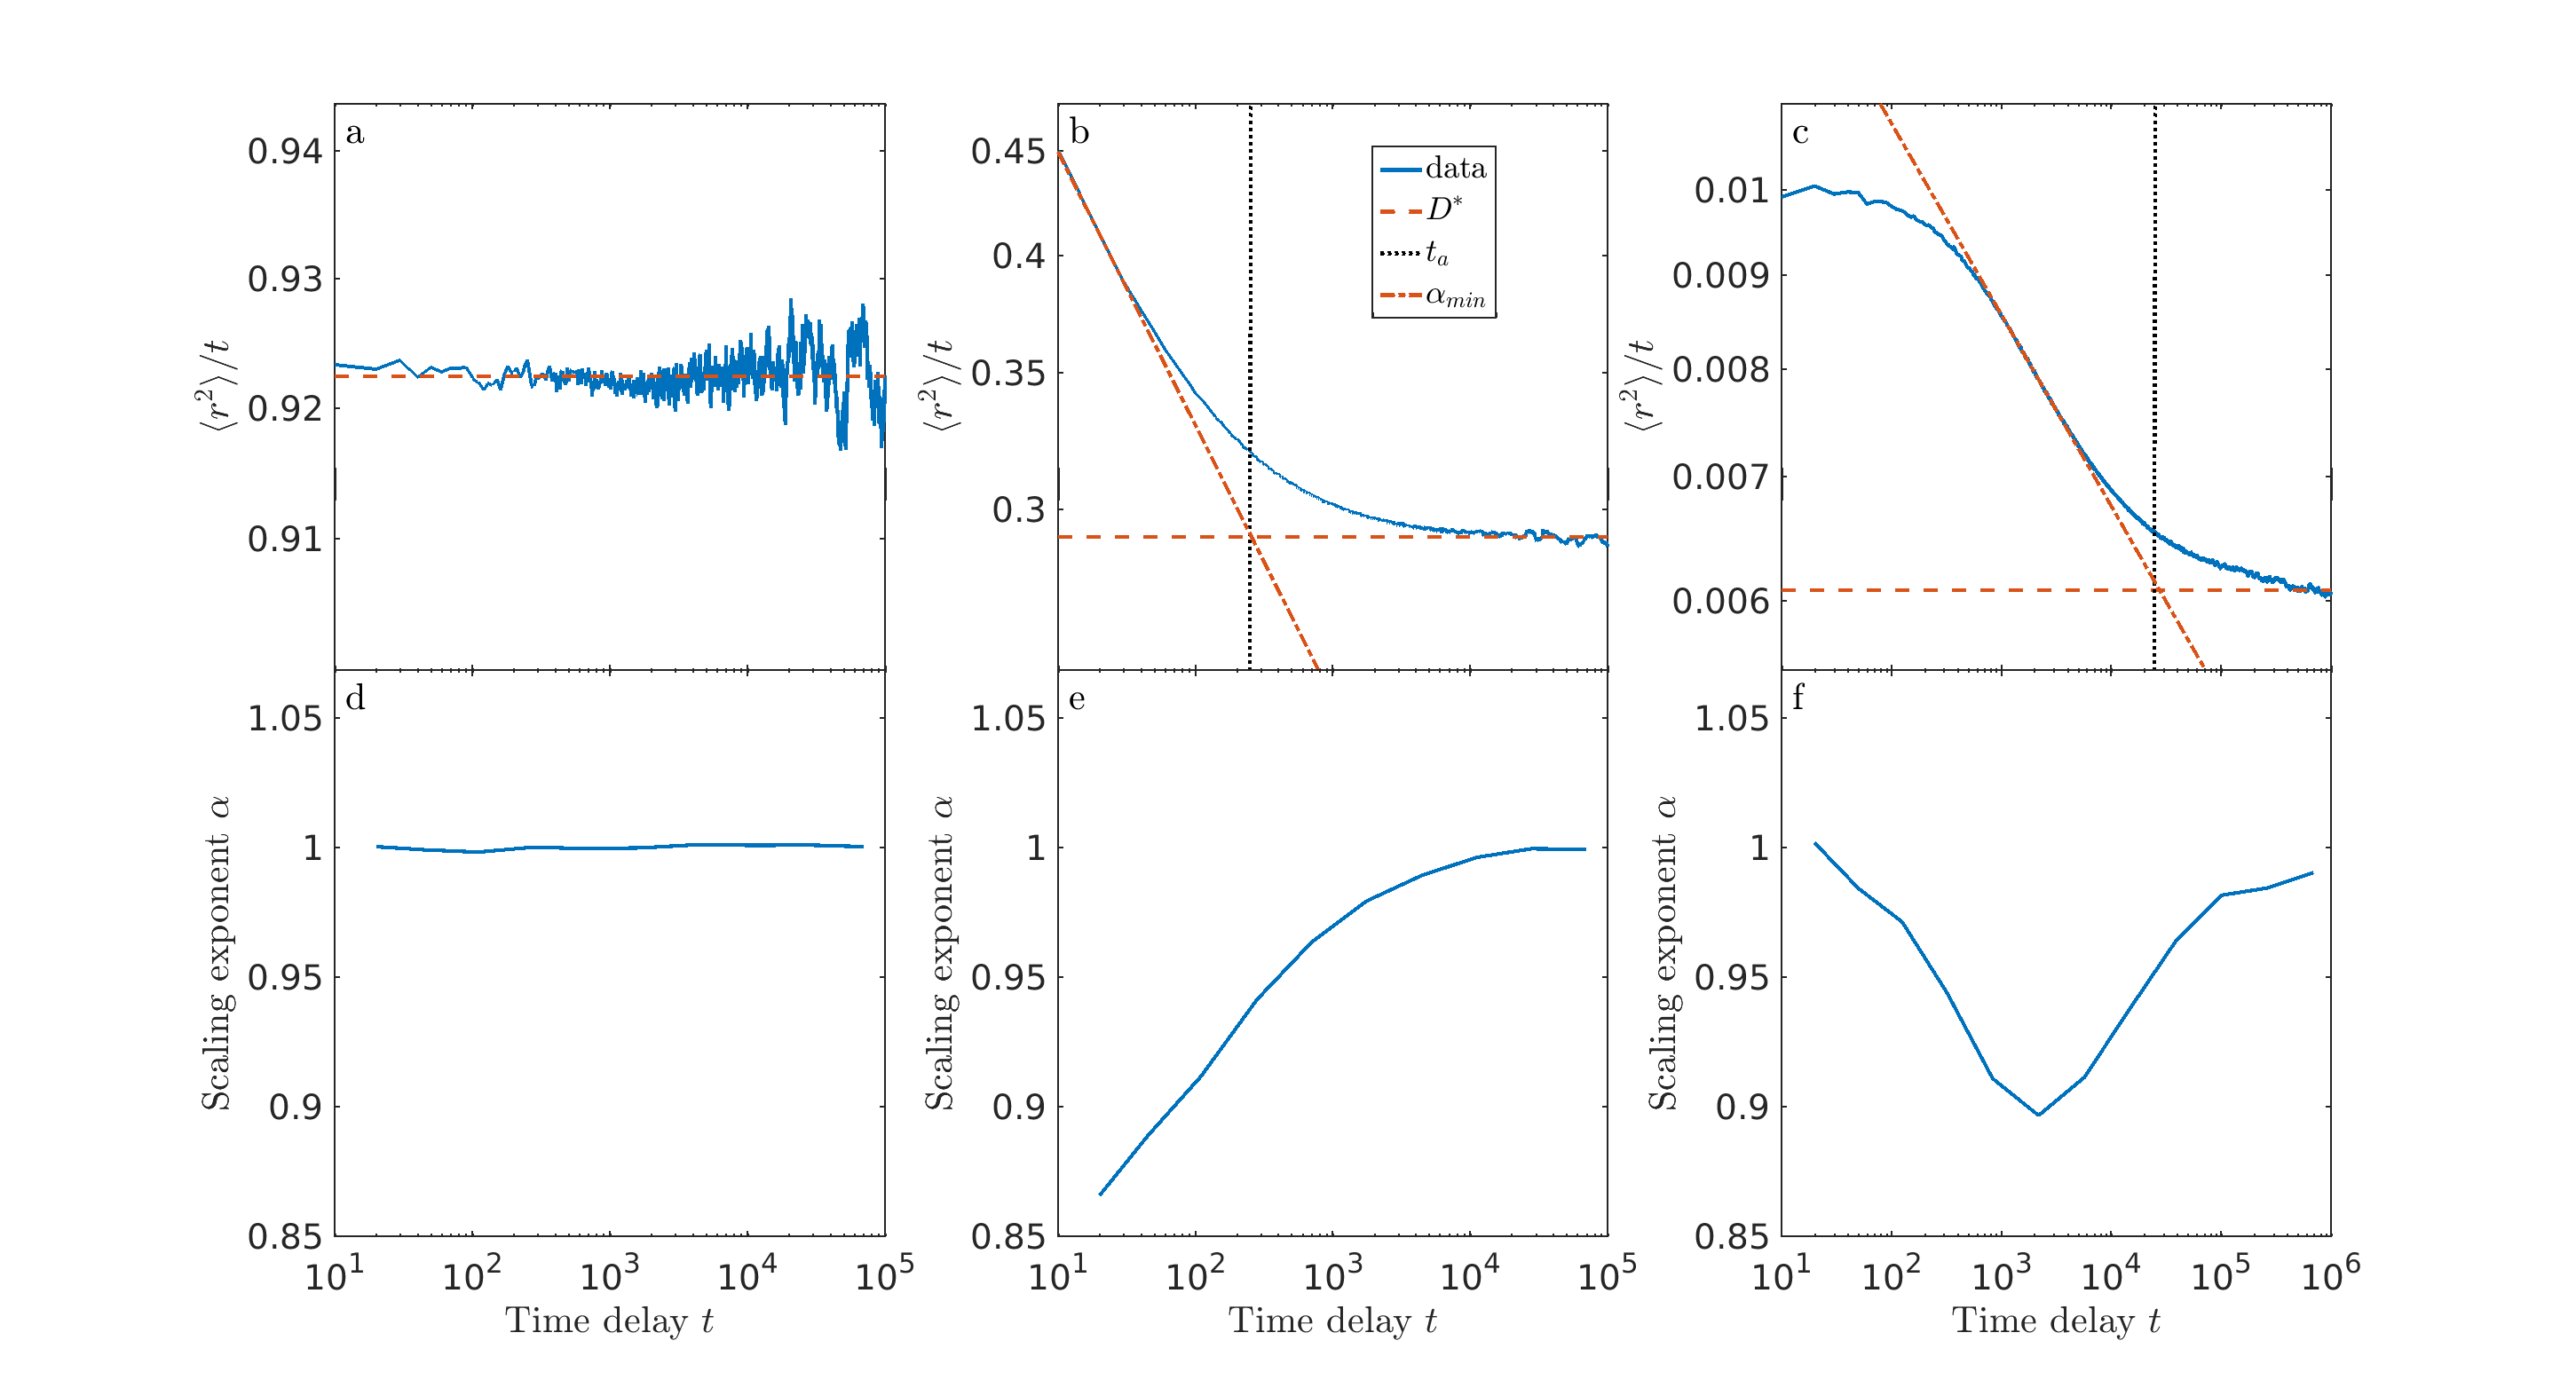
\includegraphics[width=175mm]{figs/ch02_soft/soft_msd_fits.png}
  \end{center}
	\caption[Fitting procedure]
    {Top panel: Illustration of fitting procedure, showing
    $ \langle r^2\rangle /t $ vs time delay $ t $ for simulation data (blue),
    line fitted to horizontal asymptote (red dashes), line tangent to
    point of maximum absolute slope of the curve (red dash-dots), and
    anomalous time $ t_a $ (black dots) for different
    parameters. Bottom panel: instantaneous scaling exponent
    $\alpha$ vs time delay $t$. (a, d) Slippery obstacles with $ \Delta G = 1 $,
    $ \nu = 0.95 $: normal diffusion occurs for all measured time.
    (b, e) Sticky obstacles with $ \Delta G = 2 $, $ \nu = 0.45 $.
    (c, f) Sticky obstacles with $ \Delta G = -5 $, $ \nu = 0.50 $.}\label{fig:msd_fits}
\end{figure}

For non-power law dynamics, we can apply \eqnref{eqn:msd_anom_full} locally,
with a phenomenological, time-varying exponent. Then $\alpha(t)$ is defined by
local fitting to the logarithm of $\frac{\langle r^2 \rangle}{t}$:
%
\begin{equation}
  \label{eqn:log_msd}
  \log \left( \frac{\langle r^2 \rangle}{t} \right)  
    = \log \left( 2dD  \right) + ( \alpha(t) - 1 ) \log \left( t \right),
\end{equation}
%
so that $\alpha(t) - 1 $ is the local slope of the $\frac{\langle r^2 \rangle}
{t}  $ versus $t$ curve on a log-log plot.  As seen in
figs.~\ref{fig:msd_curves} and~\ref{fig:msd_fits}, the instantaneous effective
$\alpha$ varies with delay time.  Thus, a power law MSD scaling with time, such
as can arise from fractional Brownian dynamics, does not encompass the
complexity of our crowded diffusion model, as has been found
previously~\cite{ellery_modeling_16, jeon_protein_16}.


At short times, our model typically exhibits anomalous diffusion. However, under
some conditions, the short-time behavior is diffusive, with an intermediate
anomalous regime.  We defined $\alpha_{\min}$ as the minimum instantaneous value
of $\alpha$ (the most anomalous exponent).  We characterized the transition
between short- or intermediate-time anomalous diffusion and long-time normal
diffusion by the time scale $t_a$, determined as the intersection of the
horizontal long-time asymptote of $ \frac{ \langle r^2 \rangle } { t } $  with a
line tangent to the point of the maximum rate of decrease of this curve
\figrefp[b,c]{fig:msd_fits}.  We found that this transition time could be
robustly determined for a wide range of diffusion coefficients and anomalous
behavior. We denote $t_{a}$ the anomalous time. Qualitatively, it is the
crossover time from short-time subdiffusion to long-time Fickian diffusion.
While $\alpha_{\min}$ characterizes how trapped a tracer is, $t_{a}$ quantifies
how long it takes a tracer to escape a cage and forget the memory effects that
the cage introduced to its motion.  

We defined the long-time Fickian diffusion coefficient as
%
\begin{equation}
  \label{diff}
  D = \lim_{t \to \infty} \frac{\langle r^2 \rangle} {2d t}.
\end{equation}
%
All diffusion coefficient measurements are expressed in terms of the scaled
diffusion coefficient $ D^* = \frac{ D } {D_0} $, where $ D_0 = \frac{ l^2 }{ 2
  d \tau} $ the diffusion coefficient in the absence of obstacles, $l$ the
distance between lattice sites (here defined to be 1), and $\tau$ the time
interval between steps (also set to 1).

In practice, we binned \eqnref{eqn:log_msd} into ($\sim 10$) separate regions.
We locally fit the slope of each region.  If the magnitude of the slope was
below a certain threshold value, we assumed it was flat.  We then took a
weighted averaged of all dependent values
$\log{\left(\frac{\ev{r^2}}{t}\right)}$ from the first, \textit{i.e.}, earliest
time, flat bin to the end of the simulation to calculate the horizontal
asymptote. The scaling coefficient $\alpha$ was found from the bin with the
largest negative slope, and $t_a$ was calculated from the intercept of the
horizontal asymptote and the fit line from the bin associated with $\alpha$.

In some cases, we were unable to determine all of $D^*$, $\alpha_{\min}$, and
$t_a$. For some parameter sets, the slope of $\frac{\ev{r^2}}{t}$ vs.  $ t $ on
a log-log plot approached a non-zero constant, indicating that diffusion was
anomalous over all measured time delays, so that the Fickian diffusion
coefficient was not well-defined. For other parameter sets, the
$\frac{\ev{r^2}}{t}$ versus $ t $ curve did not reached a clear asymptote during
the simulation time. We therefore could not determine $D^*$, but could measure
$\alpha_{\min}$.  When tracer diffusion was normal over all or nearly all
measured time delays, neither $\alpha_{\min}$ nor $t_a$ were well-defined, but
$D^*$ could be measured.

\section{Sticky soft obstacles}
% figure 04 %
\begin{figure}[!hb]
  \begin{center}
	  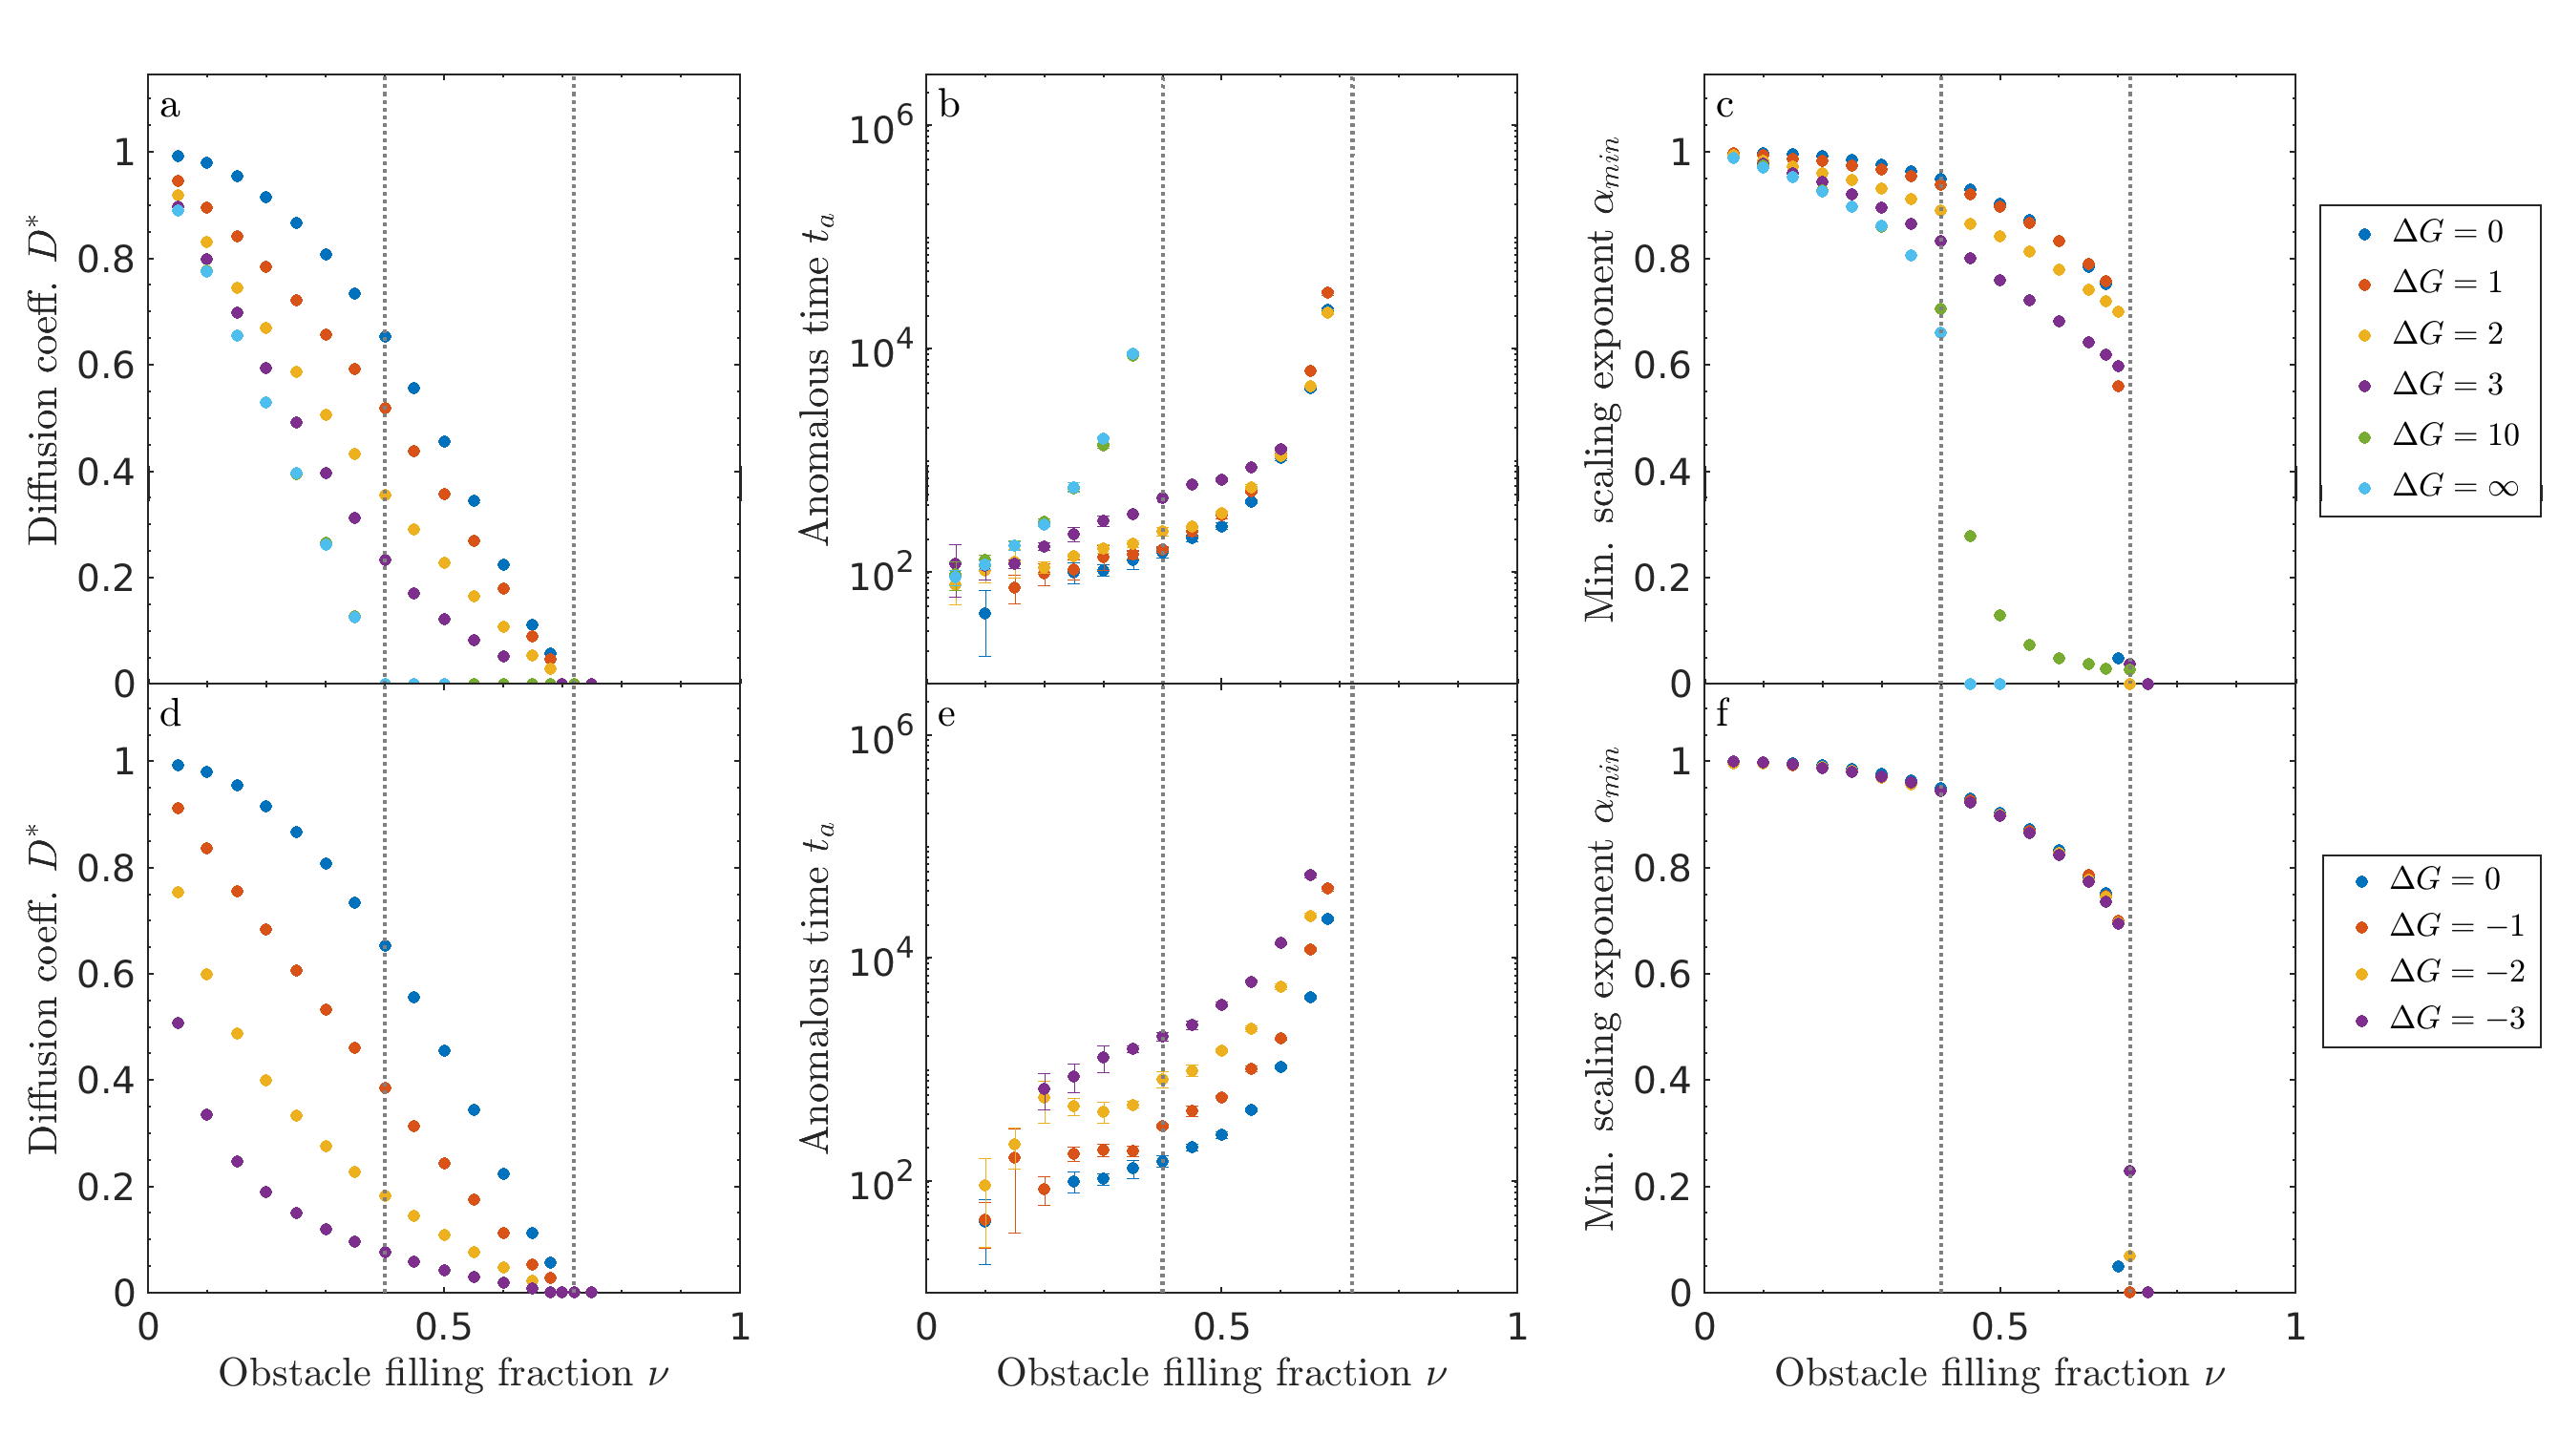
\includegraphics[width=175mm]{figs/ch02_soft/soft_sticky_2d.png}
  \end{center}
	\caption[Sticky diffusion in 2D]
    {Sticky obstacles of size one in 2D.  (a, d) Diffusion
    coefficient $D^*$, (b, e) anomalous time $ t_a $, and (c, f)
    minimum scaling exponent $\alpha_{\min}$ as a function of
    obstacle filling fraction $\nu$ for repulsive (top) and attractive
    (lower) binding energy. Note that points for $\Delta G = 10 $ are
    partially hidden behind $ \Delta G = \infty$.  The approximate
    locations of the critical occupancies $ \nu^l $ and $ \nu^u $ are
    indicated with gray dotted lines.}\label{fig:sticky_2d}
\end{figure}

% figure 05 %
\begin{figure}[!ht]
  \begin{center}
	  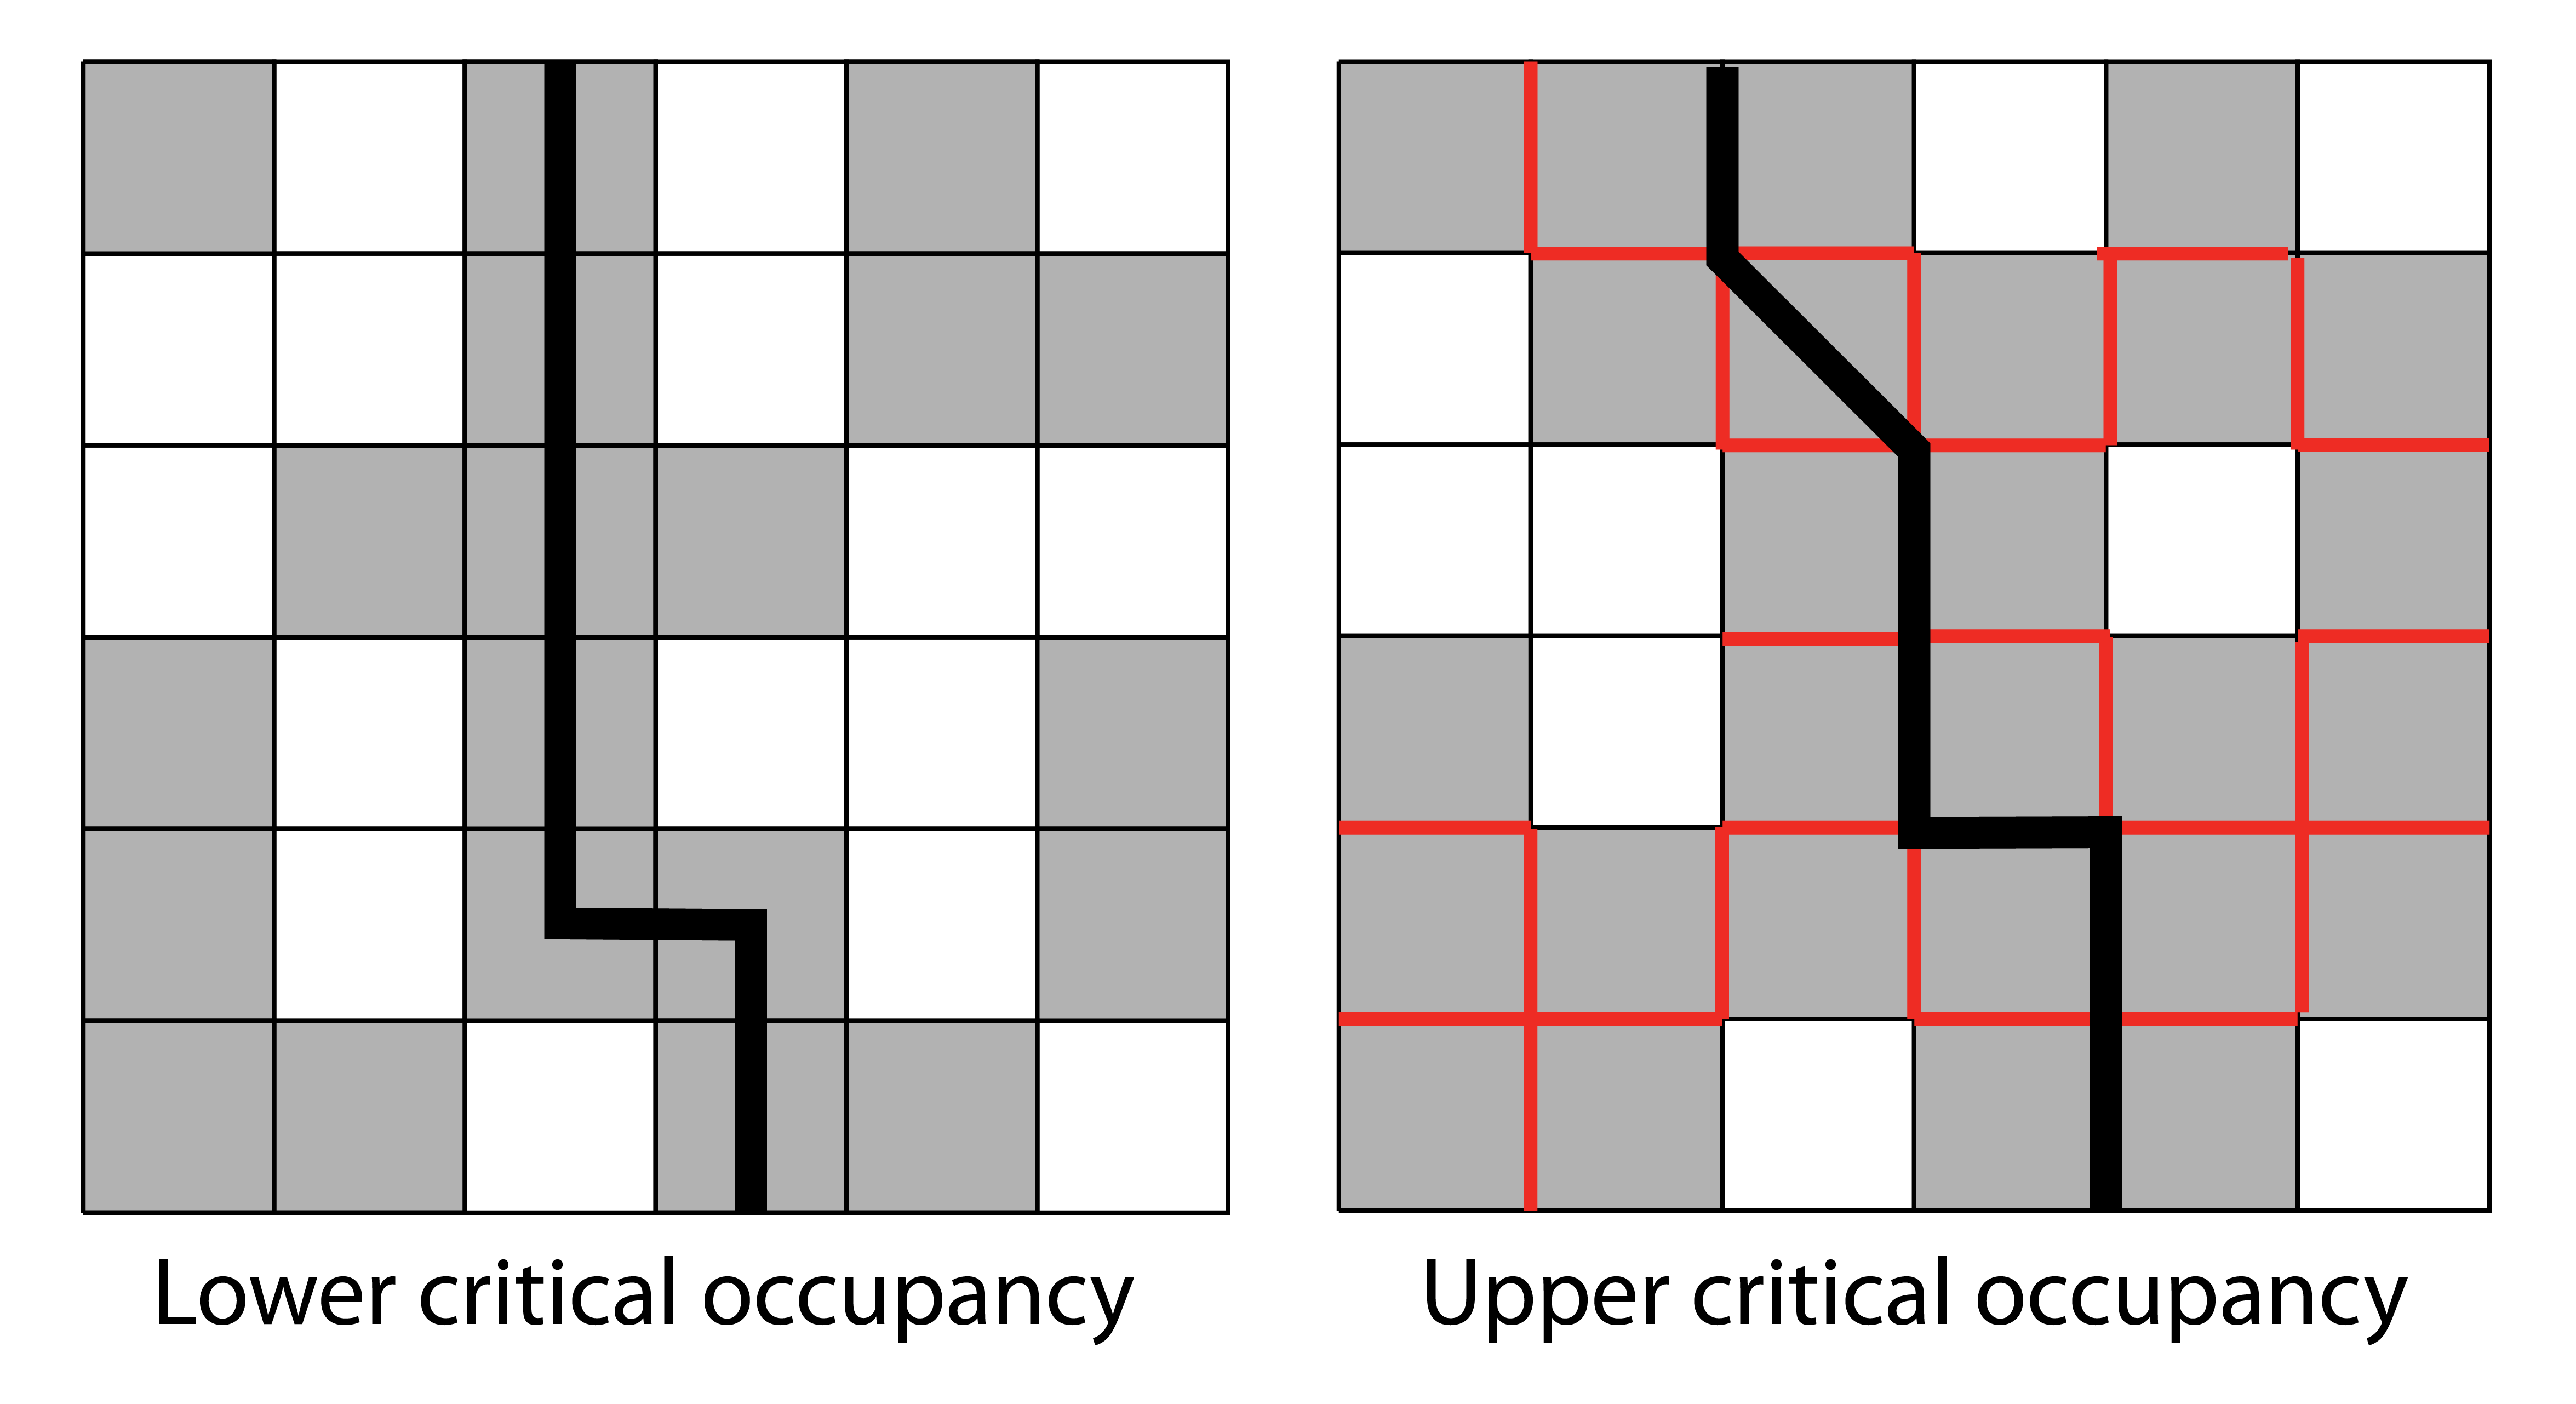
\includegraphics[width=100mm]{figs/ch02_soft/soft_percolation.png}
  \end{center}
	\caption[Percolation threshold]
    {The two types of percolation threshold in our lattice
    model: the lower critical occupancy $ \nu^l $ (left) and the upper
    critical occupancy $ \nu^u $ (right). For the lower critical
    occupancy, which is the standard percolation threshold, the
    percolating network is the obstacles. At the upper critical
    occupancy, the percolating network is the \textit{interface}
    between two or more obstacles. The barrier to tracer motion is
    shown as a black line; obstacle-obstacle boundaries which cannot
    be crossed by a tracer in the sticky model are shown in
    red. Without binding, tracers cannot pass through the 
    percolating network of obstacles. If they can bind, tracers can `hop through'
    a single obstacle, with or without bound motion.}\label{fig:percolation}
\end{figure}
% figure 05 %

We initially focused on the limit of perfectly sticky obstacles of size 1, to
determine the effects of stickiness, filling fraction, and binding energy on
tracer motion. We varied parameters over a wider range for the 2D model, with a
comparison to 3D results for some parameter sets.

For sticky obstacles, the motion of a bound tracer to an adjacent obstacle is
prohibited.  This could occur, for example, because the net free energy cost of
binding to an obstacle is a result of an attractive binding interaction, with a
high free energy barrier to moving to an adjacent site.  Here, we consider the
limit that the free energy cost of moving to an adjacent obstacle is so large
that it approaches infinity.  This situation provides an important point of
comparison to explicitly test the effects of bound-state diffusion on tracer
behavior.

We separately consider repulsive and attractive obstacles
\figrefp{fig:sticky_2d}.  Note that we include the case $\Delta G=0$, that is,
where the binding interactions are neither attractive nor repulsive, but still
block moves to adjacent obstacles.  We define the lower critical occupancy
$\nu^l$ as the filling fraction at which diffusion is non-Fickian for all time
scales for impenetrable obstacles ($\Delta G = \infty$).  In the limit of a hard
repulsive obstacle, $D^*$ decreases with filling fraction, and approaches zero
at the percolation threshold expected for hard obstacles on a square lattice,
$\nu^l \approx 0.4$~\cite{stauffer_introduction_94}, where $t_a$
diverges~\cite{saxton_lateral_87}.  The lower critical occupancy is the
percolation threshold, at which there is no longer a continuous path of empty
sites \figrefp{fig:percolation}.


For finite binding free energy in our model, Fickian diffusion can still occur
above the percolation threshold $\nu^l$ because soft binding allows tracers to
`hop through' single obstacles via binding and unbinding. Without soft binding
of the type we consider, obstacle percolation would prevent a tracer from moving
between vacancy clusters. In other words, tracers that start in an area caged by
obstacles are stuck there.  With soft binding, tracers that start in a cage can
hop onto an obstacle and then hop off into a new vacancy cluster.  For soft
binding interactions and sticky obstacles, there is an upper critical occupancy
$ \nu^u \approx 0.72 $ at which the long-time diffusion coefficient approaches
zero irrespective of binding energy \figrefp{fig:sticky_2d}. Above $\nu^u$,
tracers become caged regardless of the binding kinetics.  Therefore, there is a
different type of percolating network above the upper critical occupancy: the
percolation of the inter-obstacle boundary \figrefp{fig:percolation}.  At the
upper critical occupancy, there is a second adjacent obstacle preventing the
tracer from `hopping through.' Note that, as expected, the transition time $t_a$
appears to diverge on the approach to the upper critical occupancy
\figrefp{fig:sticky_2d}.  We are unaware of a theoretical value for this
percolating density, but our results suggest its approximate value is $0.72$ in
2D \figrefp{fig:sticky_2d}.  Intermediate repulsive binding energy leads to
intermediate behavior, as expected. For strong repulsion, \textit{e.g.}, $\Delta
G=5$, $D^*$ remains small, though clearly non-zero, up to the upper critical
occupancy, while $t_a$ monotonically increases until it diverges at $\nu^u$.

Anomalous dynamics appear in the slope of $ \langle r^2 \rangle / t $ on a
log-log plot. The most anomalous behavior occurs when the scaling coefficient $
\alpha $ reaches its smallest value, $\alpha_{\min}$.  We find that
$\alpha_{\min}$ decreases with filling fraction and binding energy
\figrefp[c]{fig:sticky_2d}. Adding more obstacles and increasing the repulsion
causes greater hindrance of tracer motion.  We note that $\alpha_{\min} \approx
0.7$ near $\nu^l$ for impenetrable obstacles, as found
previously~\cite{saxton_anomalous_94, nicolau_sources_07}.  Finite repulsive
binding energy leads to a smaller exponent ($ \alpha_{\min} < 0.7 $) than the
infinite case at filling fraction above $\nu^l$. For lower values of $\Delta G$,
the scaling coefficient does not go to zero at the upper critical occupancy $
\nu^u $.  Note that the sharp cutoff with filling fraction occurs because we did
not collect data past $ \nu^u $.

Sticky obstacles with attractive binding interactions show a more rapid falloff
in the diffusion coefficient and larger anomalous time \figrefp{fig:sticky_2d}.
The upper critical density $ \nu^u \approx 0.72 $ is in the same vicinity as for
$\Delta G > 0$.  The dependence of the diffusion coefficient on filling fraction
for positive and negative binding energy are similar for low magnitude of the
binding energy, but the diffusion coefficient falls off more rapidly with
filling fraction for highly attractive obstacles. This occurs because an
attractive obstacle confines a tracer in one position until it escapes, while a
repulsive obstacle only impedes tracer motion for one time step. Therefore,
repulsive interactions require several obstacles to transiently confine a
tracer, while a single attractive obstacle can cause confinement. Note that we
did not include large attractive binding free energy in our analysis.

For attractive obstacles, $ \alpha_{\min} $ is independent of binding energy
over the range we studied \figrefp{fig:sticky_2d}. The characteristic time for a
tracer to unbind from an attractive obstacle depends on the binding energy,
leading to the energy-dependent variation in the anomalous time we observe.
However, it is properties of the obstacle arrangement, rather than of binding,
which determine the shape of the MSD curve, and therefore $\alpha_{\min}$.  The
minimum anomalous exponent occurs when tracers are, on average, confined to a
cage formed by inter-obstacle boundaries and single-site wells.  Therefore, the
minimum anomalous exponent is approximately the same for all binding energies, but
varies with filling fraction.

We note that the sticky soft obstacle model studied here does not simply map to
impenetrable obstacles at a lower effective obstacle filling fraction, because
tracers can `hop through' single obstacles via binding, while never being able
to hop between obstacles.  Sticky obstacles allow for move attempts (and blocks)
that would never be attempted in the impenetrable case.
% figure 06 %
\begin{figure}[!hb]
  \begin{center}
	  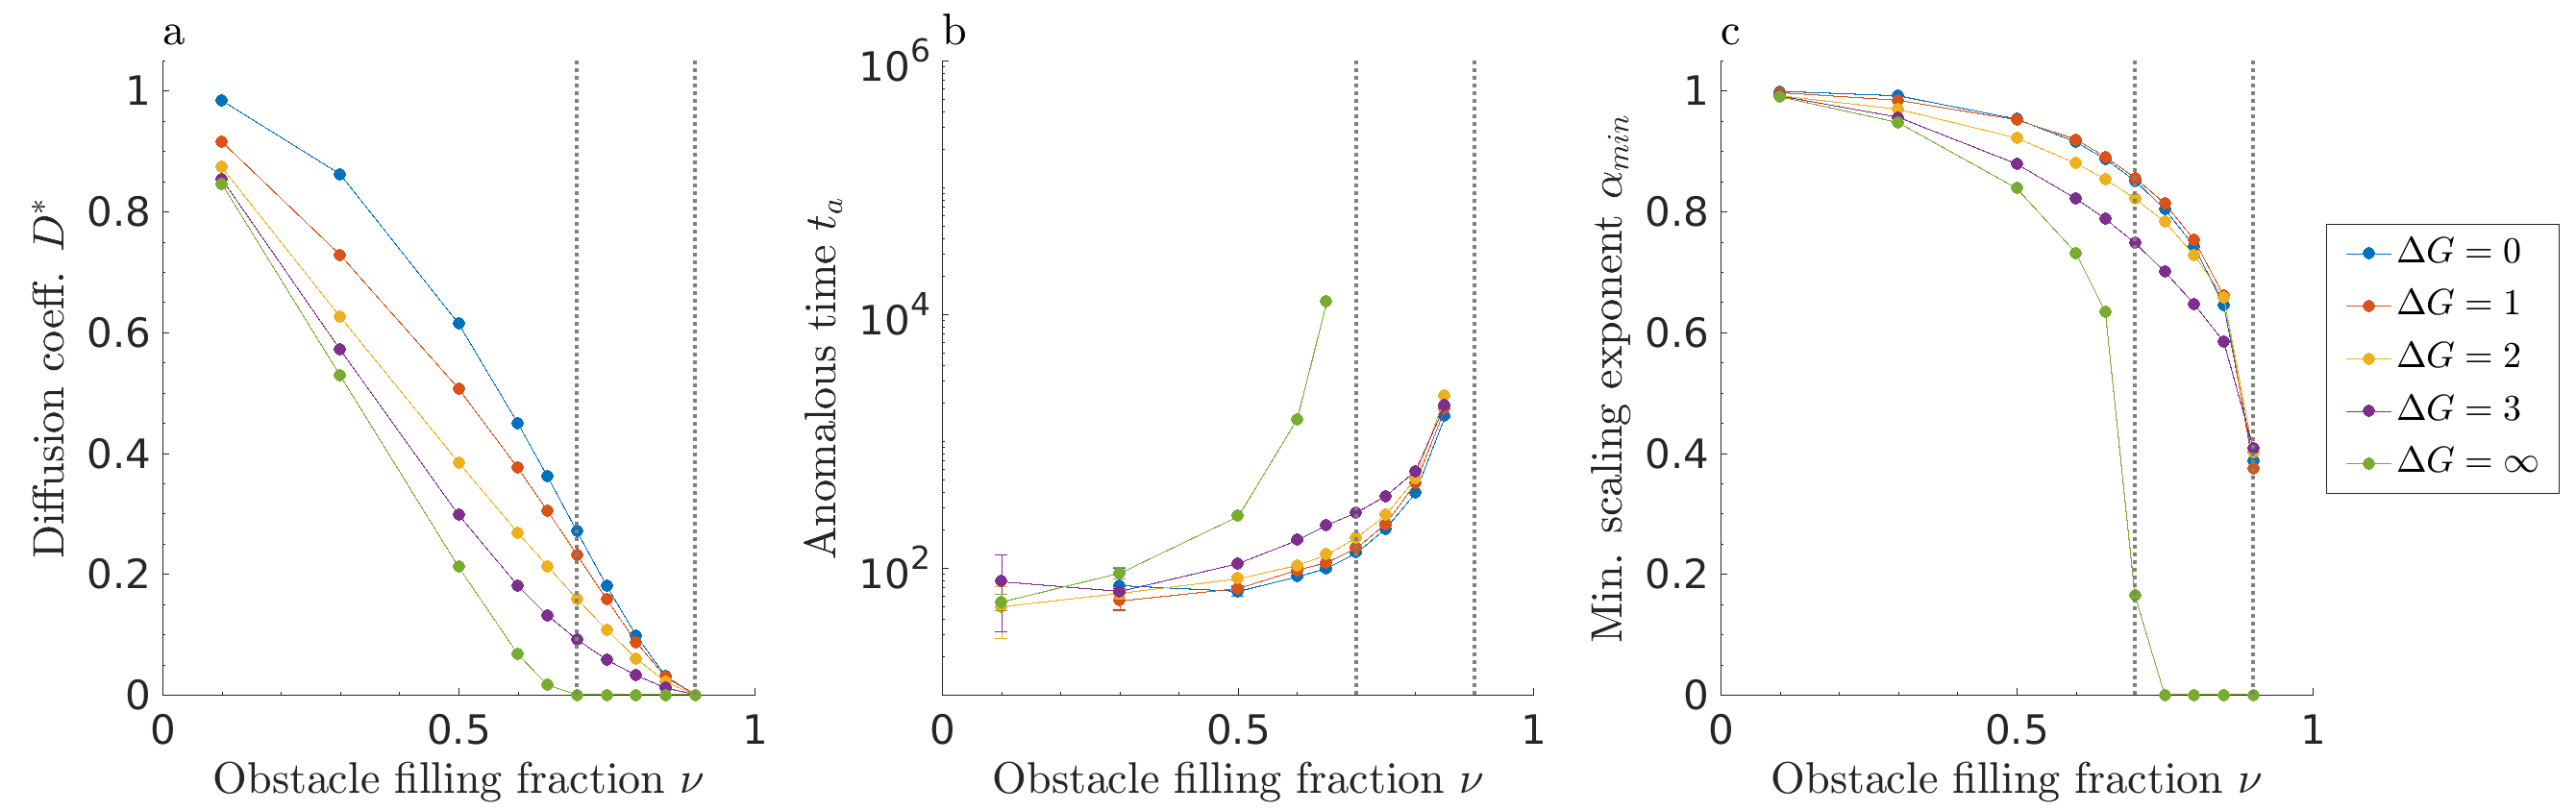
\includegraphics[width=150mm]{figs/ch02_soft/soft_sticky_3d.png}
  \end{center}
	\caption[Sticky diffusion in 3D]
    {Sticky obstacles of size one in 3D. (a) Diffusion
    coefficient $D^*$, (b) anomalous time $ t_a $, and (c) minimum
    scaling exponent $\alpha_{\min}$ as a function of obstacle
    filling fraction. The approximate locations of the critical
    occupancies $ \nu^l $ and $ \nu^u $ are indicated with gray dotted
    lines.}\label{fig:sticky_3d}
\end{figure}
% end figure 6

\subsection{Sticky soft obstacles in 3D}

We extended our study of single-site sticky repulsive obstacles to three
dimensions, to determine whether the spatial dimension plays a key role in the
tracer behavior \figrefp{fig:sticky_3d}. The results are qualitatively the same
as the 2D model \figrefp{fig:sticky_2d}.  However, in 3D, the lower and upper
critical occupancies appear at higher filling fraction: a higher obstacle
filling fraction is required to percolate a 3D lattice. The anomalous time is
also typically smaller in 3D. For sticky soft obstacles, increasing the spatial
dimension does not change the qualitative features of our model, but does shift
the critical occupancy and anomalous time.

\section{Slippery soft obstacles}

When obstacles are perfectly slippery, bound tracers can hop to adjacent
obstacles without penalty.  Our model of perfectly slippery obstacles contains
an occupancy-energy inversion symmetry: the dynamics are invariant to changing
the filling fraction by switching obstacles and empty sites ($ \nu \rightarrow
1-\nu $) while simultaneously switching the sign of the binding energy ($ \Delta
G \rightarrow - \Delta G $). In other words, a low filling fraction of
attractive obstacles is equivalent to a high filling fraction of repulsive
barriers \figrefp{fig:slippery_2d}.

% figure 07 %
\begin{figure}[!ht]
  \begin{center}
	  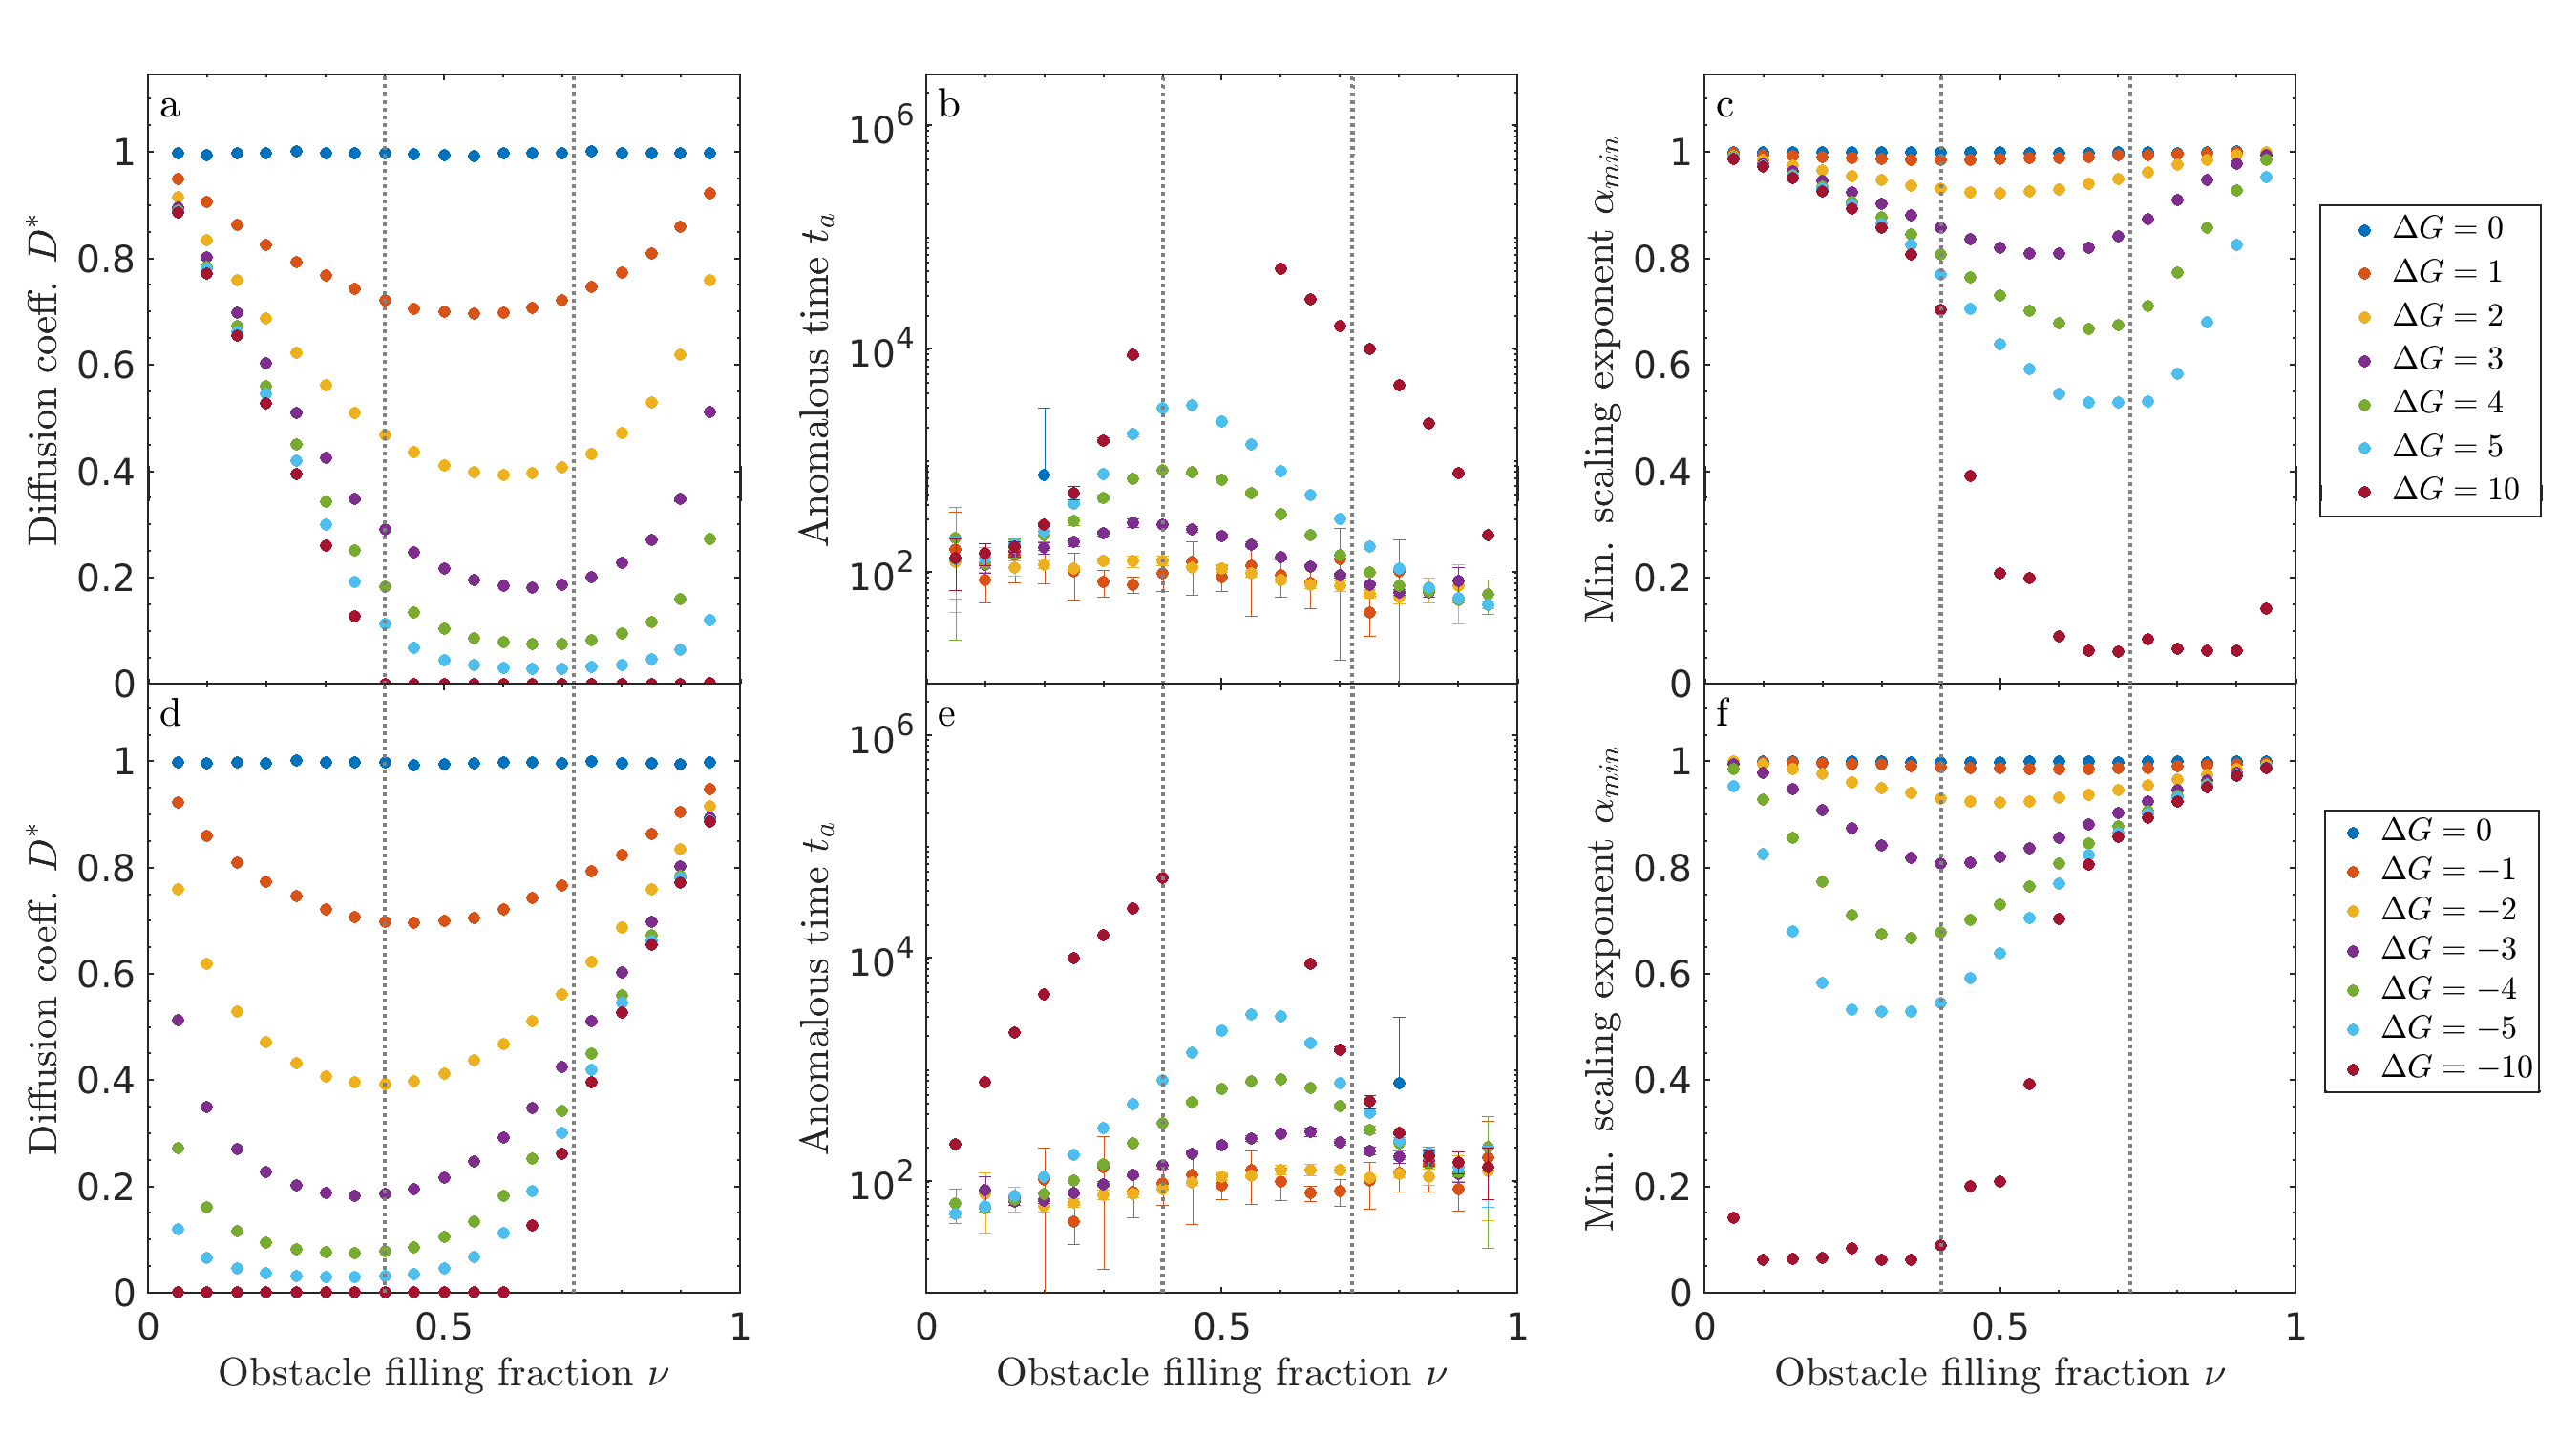
\includegraphics[width=150mm]{figs/ch02_soft/soft_slippery_2d.png}
  \end{center}
	\caption[Slippery diffusion in 2D]
    {Slippery obstacles in 2D. (a, d) Diffusion coefficient
    $D^*$, (b, e) anomalous time $ t_a $, and (c, f) minimum scaling
    exponent $\alpha_{\min}$ as a function of obstacle filling
    fraction $\nu$ for repulsive (top) and attractive (lower) binding
    energy.  The approximate locations of the critical occupancies
    $ \nu^l $ and $ \nu^u $ are indicated with gray dotted lines.}\label{fig:slippery_2d}
\end{figure}
% figure 07 %

Slippery obstacles remove the obstacle percolation threshold for all measured
binding energy \figrefp{fig:slippery_2d}. The curves for $\Delta G = 10$ for the
repulsive slippery obstacles qualitatively resemble the sticky case
\figrefp{fig:sticky_2d}, because the diffusion coefficient approaches zero for
$\nu \approx 0.4 $. However, for slippery obstacles, the anomalous time
increases, but does not diverge, at the percolation threshold, and then
decreases at larger filling fraction. For slippery obstacles with finite $\Delta
G$, one can always find a time after which the system displays normal diffusion.

Slippery obstacles lead to non-monotonic behavior: for large enough $\nu$, the
diffusion coefficient increases and anomalous time decreases. For high obstacle
filling fraction, binding increases tracer mobility, because tracers can hop
along the percolating network of obstacles.  Similarly, the minimum exponent
varies non-monotonically with filling fraction. 

\subsection{Slippery soft obstacles in 3D}

As for sticky obstacles, we examined tracer motion with single-site slippery
obstacles in three dimensions \figrefp{fig:slippery_3d}. The results are
qualitatively the same as the 2D model \figrefp{fig:slippery_2d}, with typically
smaller anomalous time.  The occupancy-energy inversion symmetry noted above for
two dimensions also holds in three dimensions. Therefore, the behavior for
attractive obstacles can be extracted from \figref{fig:slippery_3d}.

% figure 08 %
\begin{figure}[!ht]
  \begin{center}
	  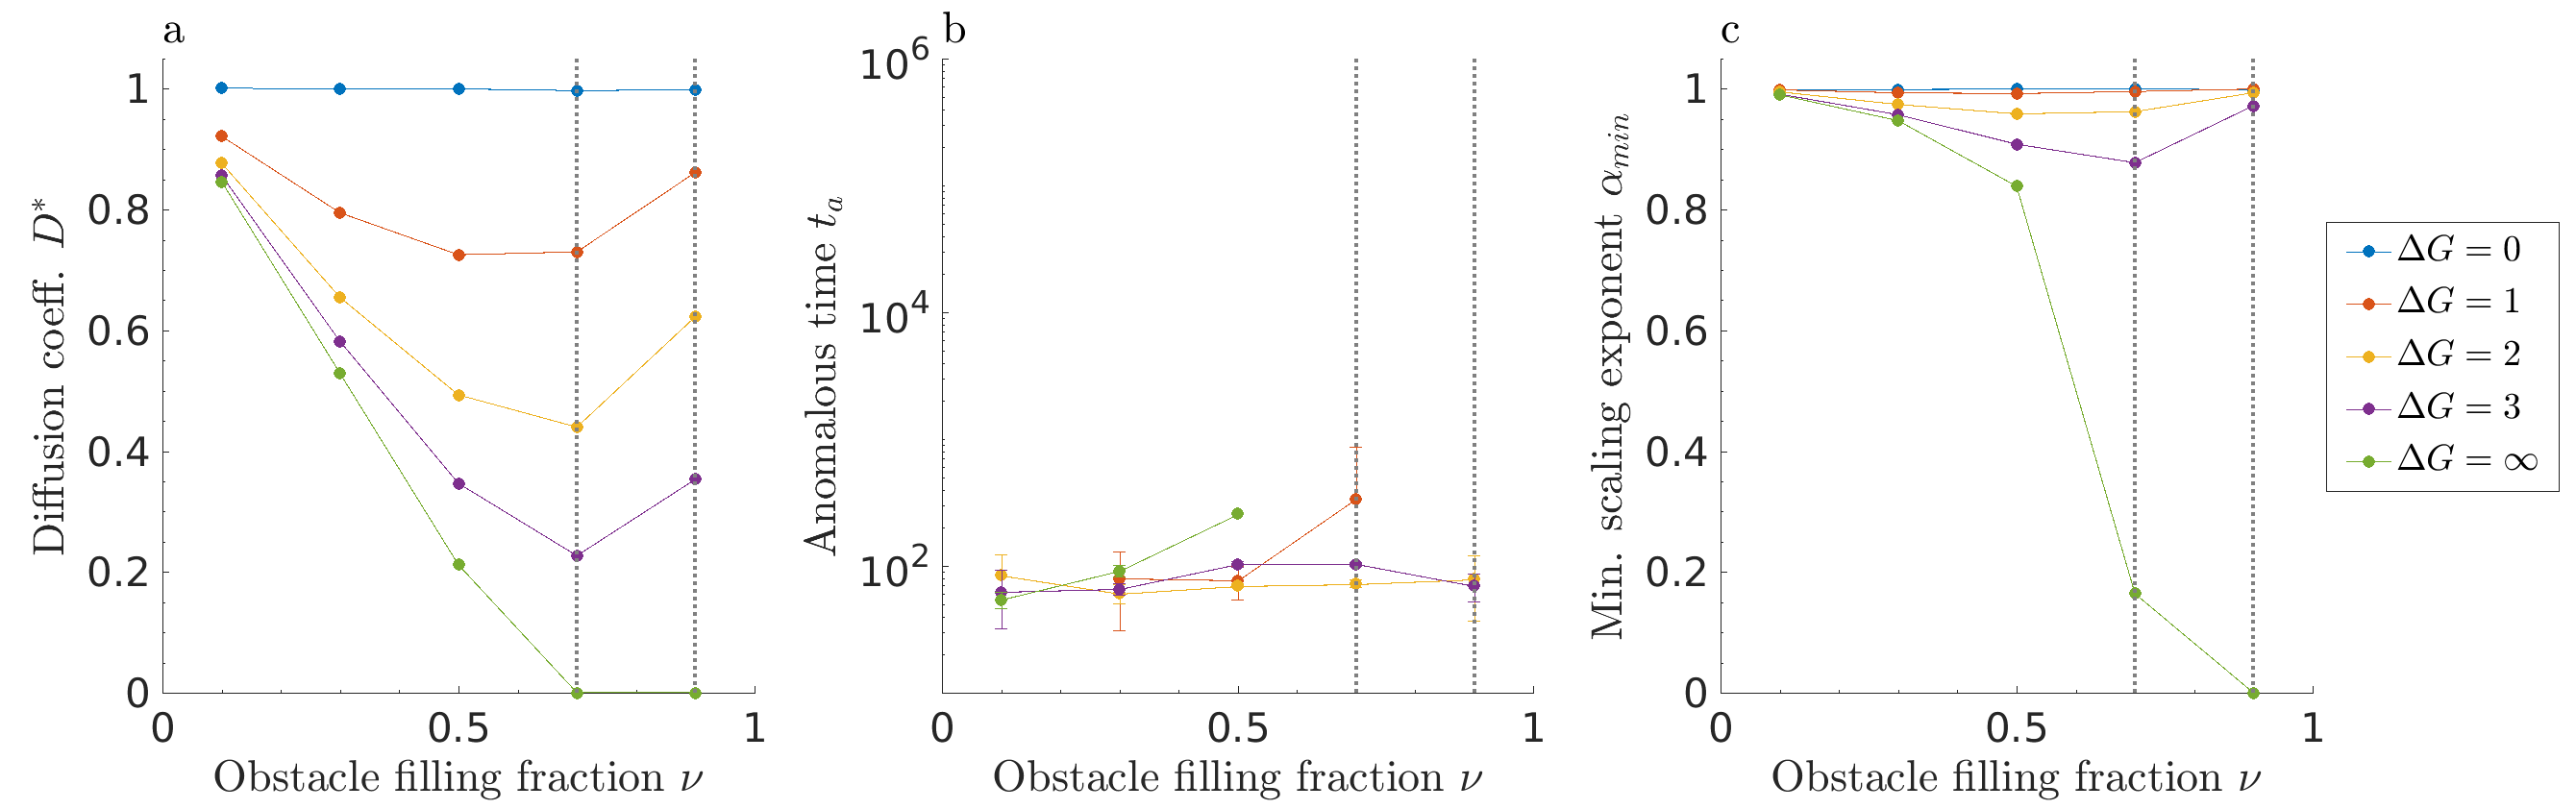
\includegraphics[width=150mm]{figs/ch02_soft/soft_slippery_3d.png}
  \end{center}
	\caption[Slippery obstacles in 3D]
    {Slippery obstacles of size one in 3D. (a) Diffusion
    coefficient $D^*$, (b) anomalous time $ t_a $, and (c)
    minimum scaling exponent $\alpha_{\min}$ as a function of
    obstacle filling fraction $\nu$. The approximate locations of the critical
    occupancies $ \nu^l $ and $ \nu^u $ are indicated with gray dotted
    lines. }\label{fig:slippery_3d}
\end{figure}
% figure 08

\subsection{Comparison of sticky and slippery obstacles in 2D}
% figure 09 %
\begin{figure}[!hb]
  \begin{center}
	  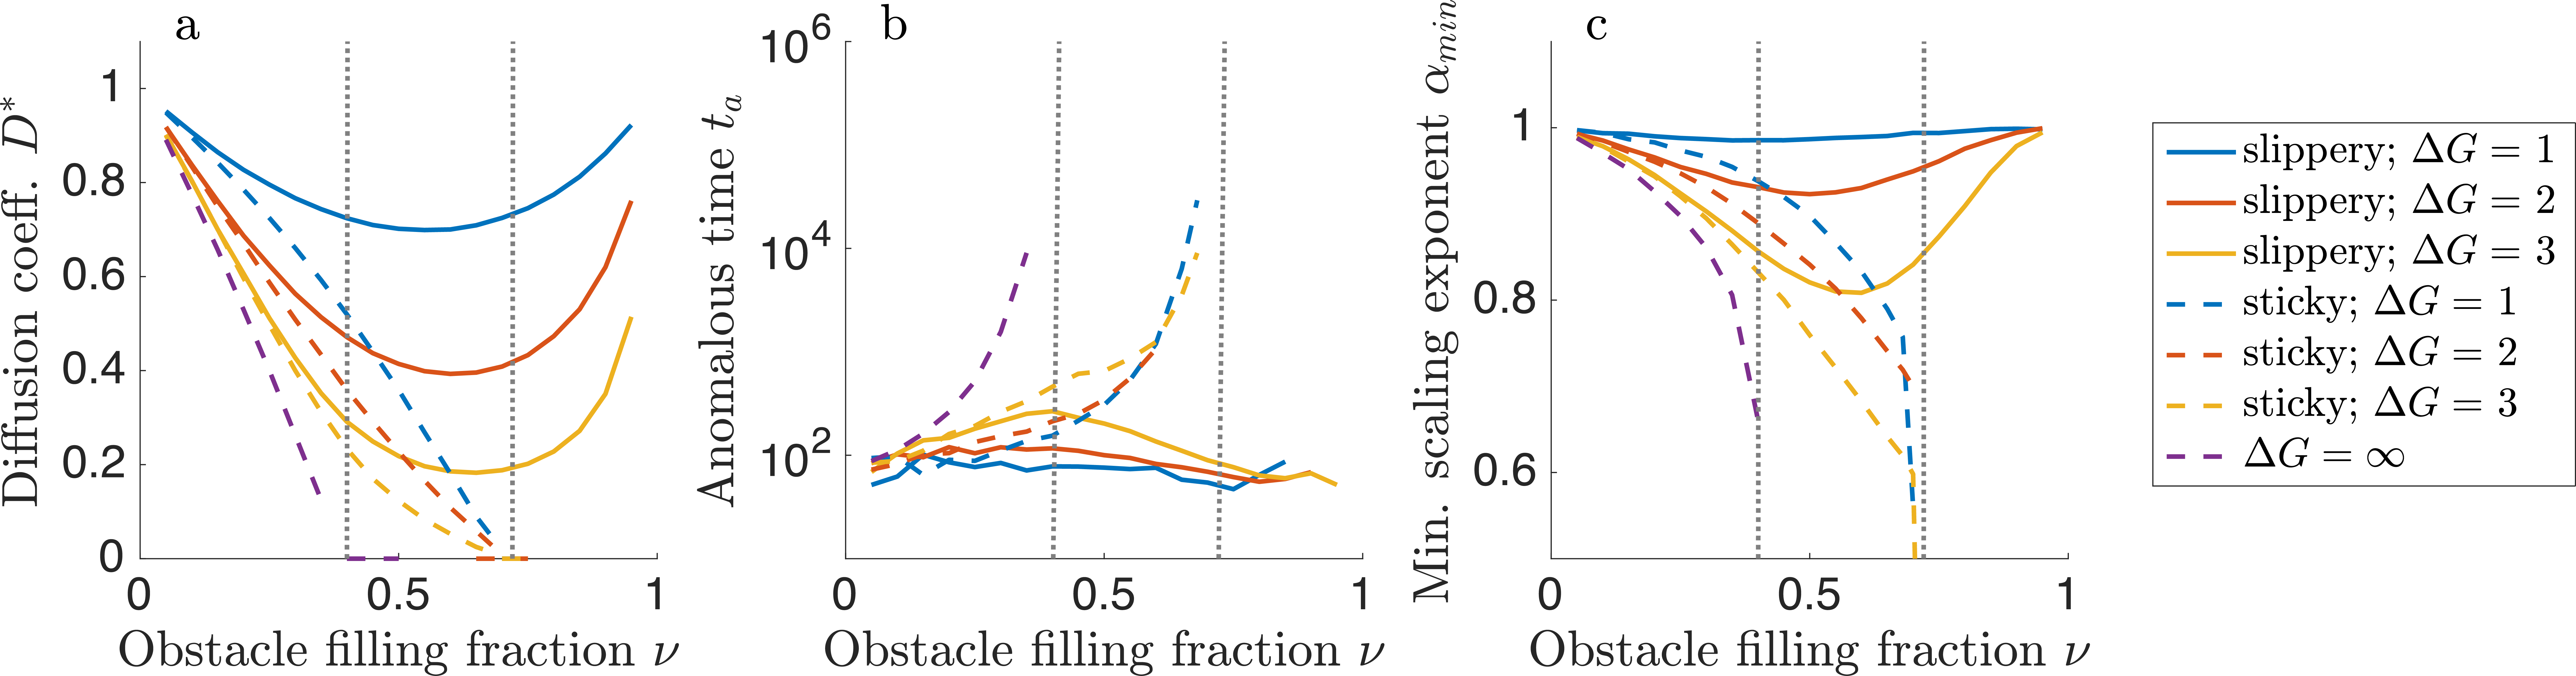
\includegraphics[width=150mm]{figs/ch02_soft/soft_compare.png}
  \end{center}
	\caption[Comparision]
    {Comparison of models with slippery repulsive obstacles
    (solid lines), sticky repulsive obstacles (dashed lines), and hard
    repulsive obstacles (purple dashed line). (a) Diffusion
    coefficient $D^*$, (b) anomalous time $ t_a $, and (c) minimum
    scaling exponent $\alpha_{\min}$ as a function of obstacle filling
    fraction $\nu$.  The gray dotted lines indicate the
    approximate locations of the critical occupancies $ \nu^l $ and
    $ \nu^u $.}\label{fig:compare}
\end{figure}
% figure 09

The limits of perfectly sticky and slippery obstacles are most similar at low
filling fraction \figrefp{fig:compare}. In general, slippery obstacles lead to
exponents closer to one (less anomalous) than do sticky obstacles, because
tracers are not caged by the obstacle-obstacle interface.  Even for relatively
small values of the binding energy ($|\Delta G| \le 3$) and intermediate filling
fraction, sticky and slippery obstacles lead to significantly different tracer
dynamics \figrefp{fig:compare}. Slippery obstacles, on which motion can occur
for high obstacle filling fraction, allow normal diffusion with coefficients
comparable to those for low filling fraction. This effect may be important to
explain the rates of a number of biological processes that are
diffusion-limited, including transcriptional regulation and nucleo-cytoplasmic
transport.
%%%%%%%%%%%%% SEMI-SLIPPERY %%%%%%%%%%%%%%%%%%%%%%%%
\section{Semi-slippery obstacles}
% figure 10 %
\begin{figure}[!hb]
  \begin{center}
	  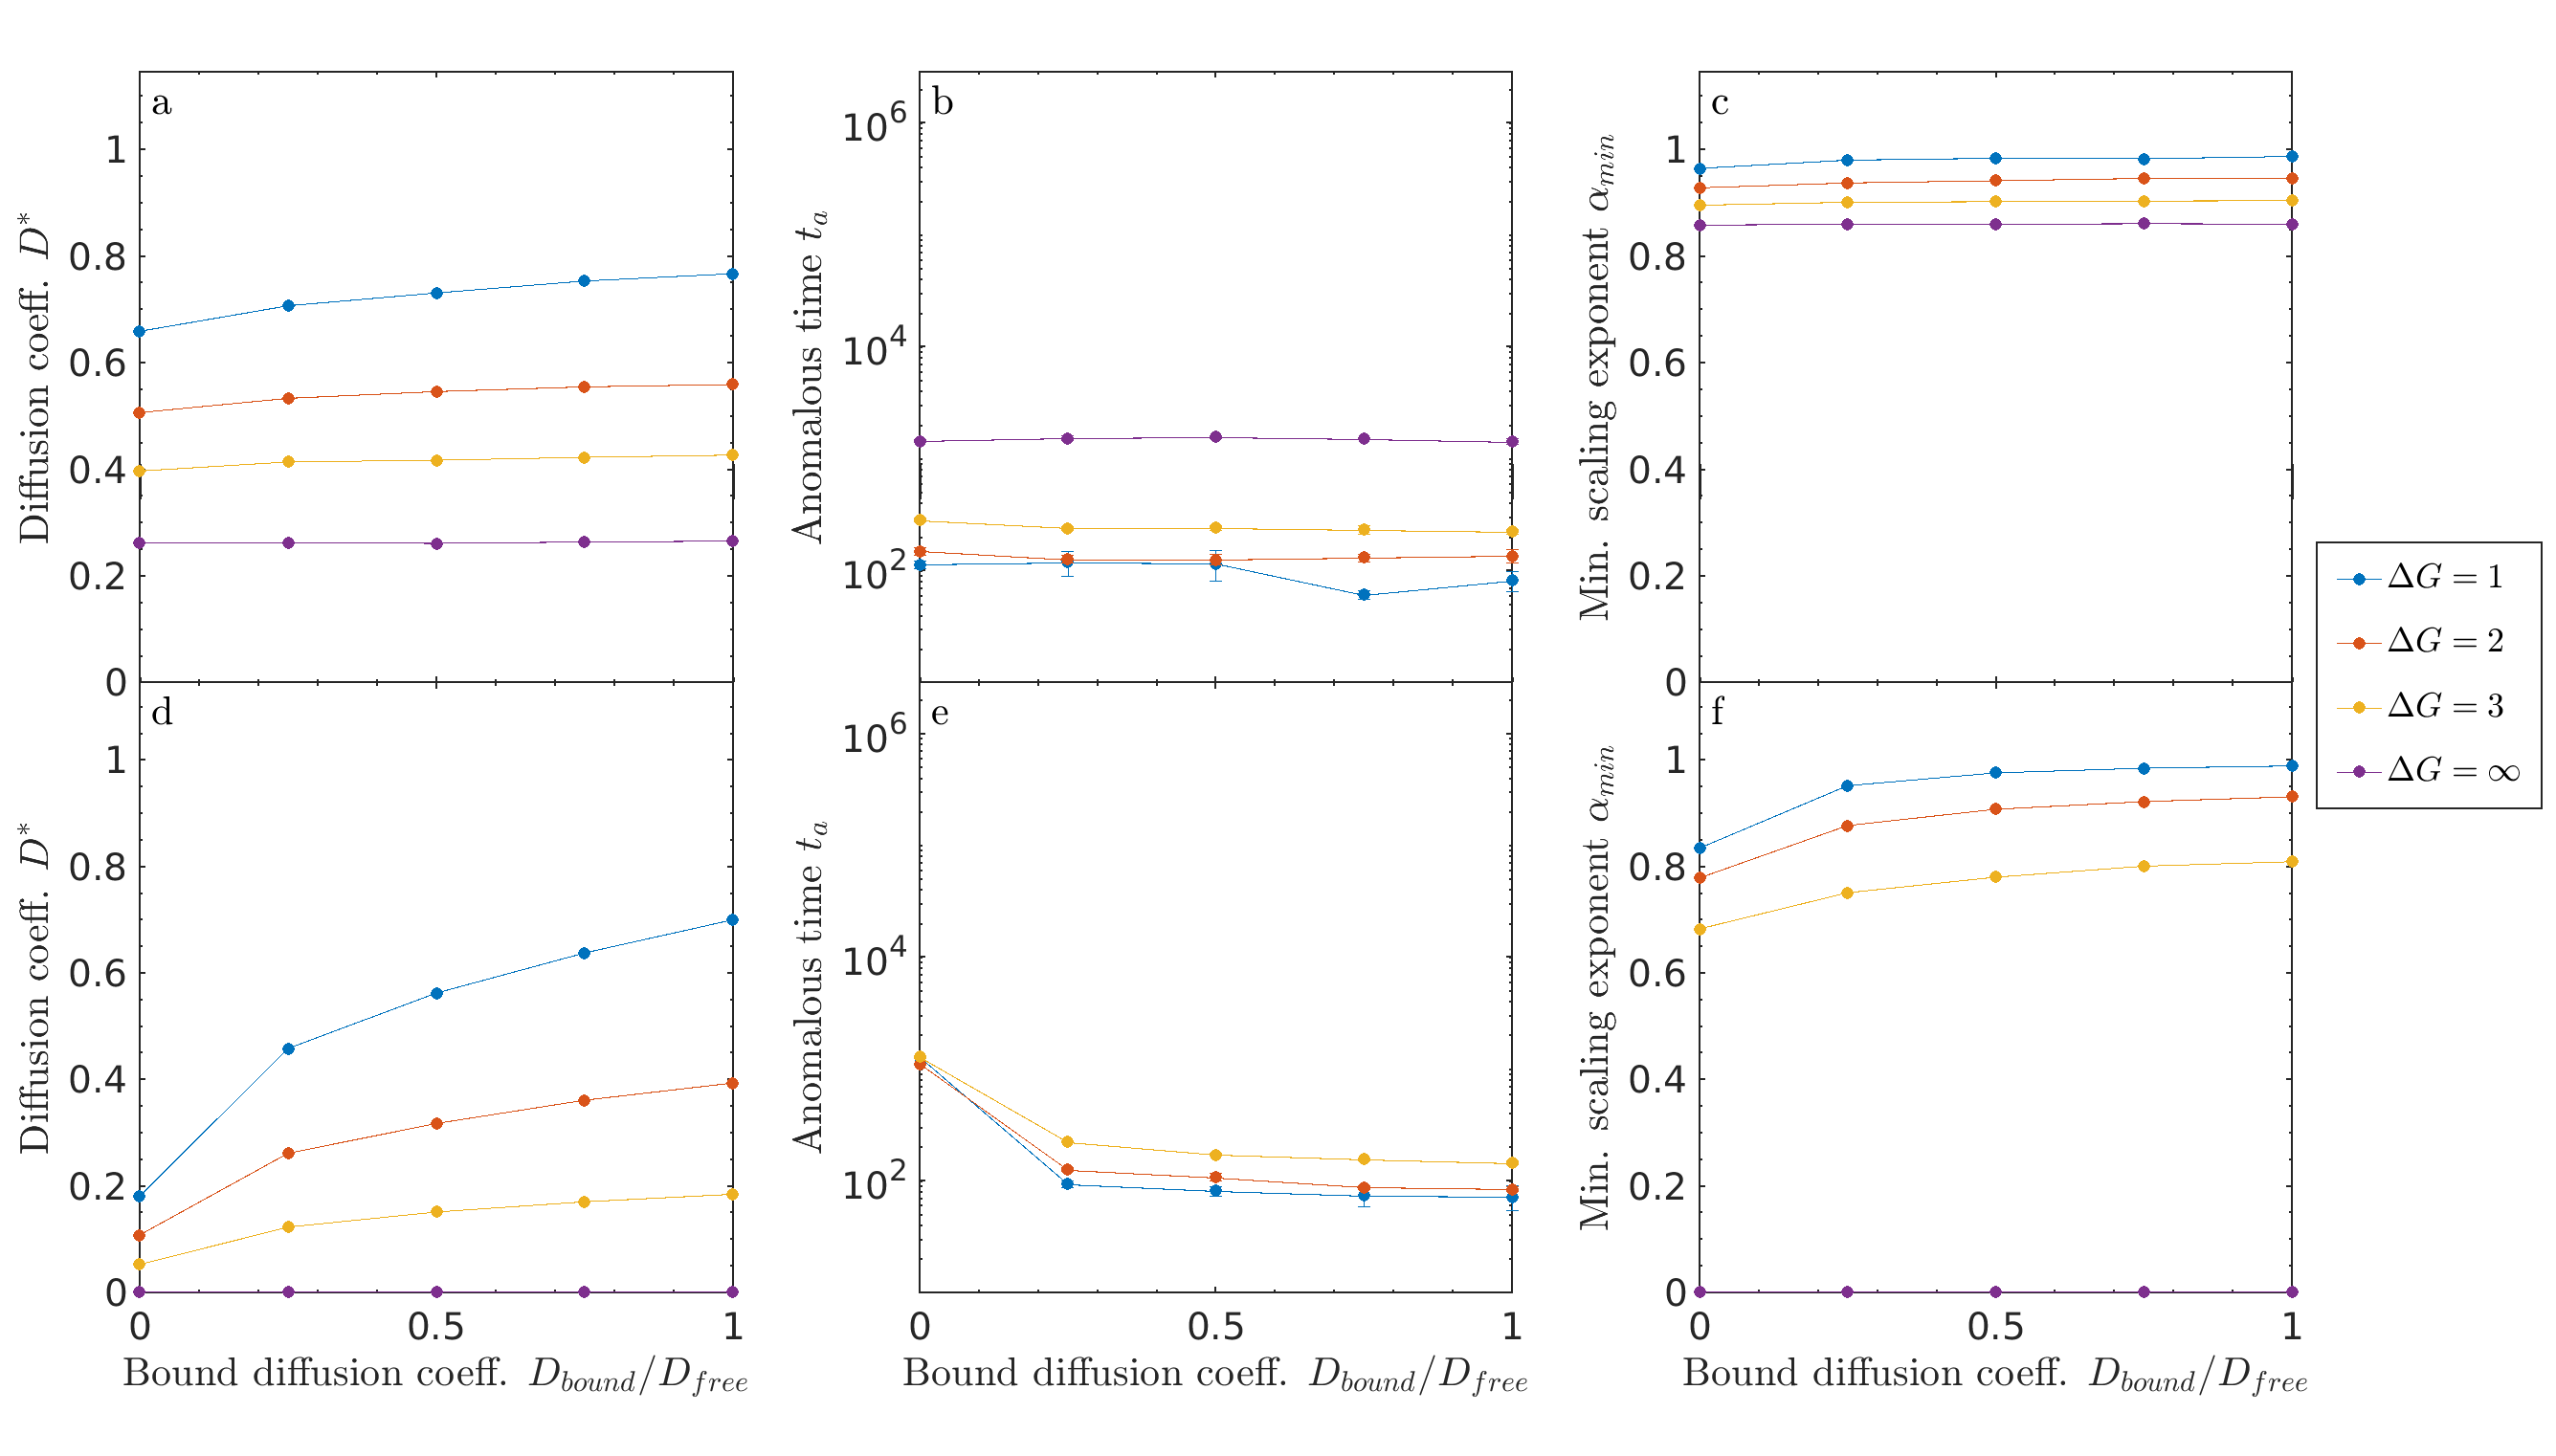
\includegraphics[width=150mm]{figs/ch02_soft/soft_semi_slippery.png}
  \end{center}
	\caption[Semi-slippery obstacles]
    {Semi-slippery obstacles in 2D.  We varied the bound diffusion
    coefficient from the sticky limit $D_{\rm bound}=0$ to the slippery
    limit $D_{\rm bound}=D_{\rm free}$ for single site obstacles.  
    (a, d) Diffusion coefficient $D^*$, (b, e) anomalous time $ t_a $, 
    and (c, f) minimum scaling exponent $\alpha_{\min}$  as function of 
    $D_{\rm bound}$ for  low filling fraction $\nu=0.3$ (top) and high 
    filling fraction $\nu =0.6$ (bottom).}\label{fig:semi_slippery}
\end{figure}
% figure 10 %

Having compared the limits of perfectly sticky ($D_{\rm bound} = 0$) and
slippery ($D_{\rm bound} = D_{\rm free}$) obstacles, we now study intermediate
cases.  We varied the bound diffusion coefficient for repulsive binding energy
$\Delta G = 1, 2, 3, \infty$ and filling fraction $ \nu = 0.3 $ and $ 0.6 $. We
chose these values to illustrate how our results change from the sticky to the
slippery case, as shown in \figref{fig:compare}.  For finite binding energy,
increasing $D_{\rm bound}$ increases the long-time diffusion coefficient
\figrefp{fig:semi_slippery}. This effect is larger for higher filling fraction
and lower binding energy, when tracers spend more time bound.  Varying $D_{\rm
  bound}$ has little effect on the anomalous time at low filling fraction,
because $t_{a}$ is already near the threshold at which we can accurately measure
it. However, increasing $D_{\rm bound}$ decreases $t_{a}$ at higher filling
fraction, because tracers can more quickly escape obstacles when their bound
diffusion coefficient is larger. Similarly, varying $ D_{\rm bound} $ has little
effect on $\alpha_{\min}$ at low $\nu$, but does make diffusion less anomalous
at higher filling fraction, because increasing bound mobility reduces tracer
caging.

\section{Varying obstacle size}

We varied the length of the obstacles $l_{\rm obst}$, while maintaining their
square shape.  Increasing the obstacle size (with filling fraction fixed)
clusters obstacles.  Since in our model the binding penalty occurs only for $
\mathbf {empty} \rightarrow \mathbf {obstacle} $ moves, increasing the size of
obstacles effectively reduces the number of binding sites: more obstacle sites
are interior to obstacles, rather than on their perimeter.  For sticky obstacles
with $l_{obst} = 1$, tracers can easily hop through cages, since their bound
motion is only blocked by an obstacle-obstacle interface.  Increasing the
obstacle size guarantees that individual obstacles will contain an
obstacle-obstacle interface, which makes it less likely that tracers can hop
through neighboring obstacles \figrefp{fig:size_moves}.  Increasing obstacle
size at fixed filling fraction also increases the typical distance between
obstacles. These changes alter obstacle percolation effects: $\nu^l$ and $\nu^u$
depend on $l_{\rm obst}$.

% figure 11 %
\begin{figure}[b]
  \begin{center}
	  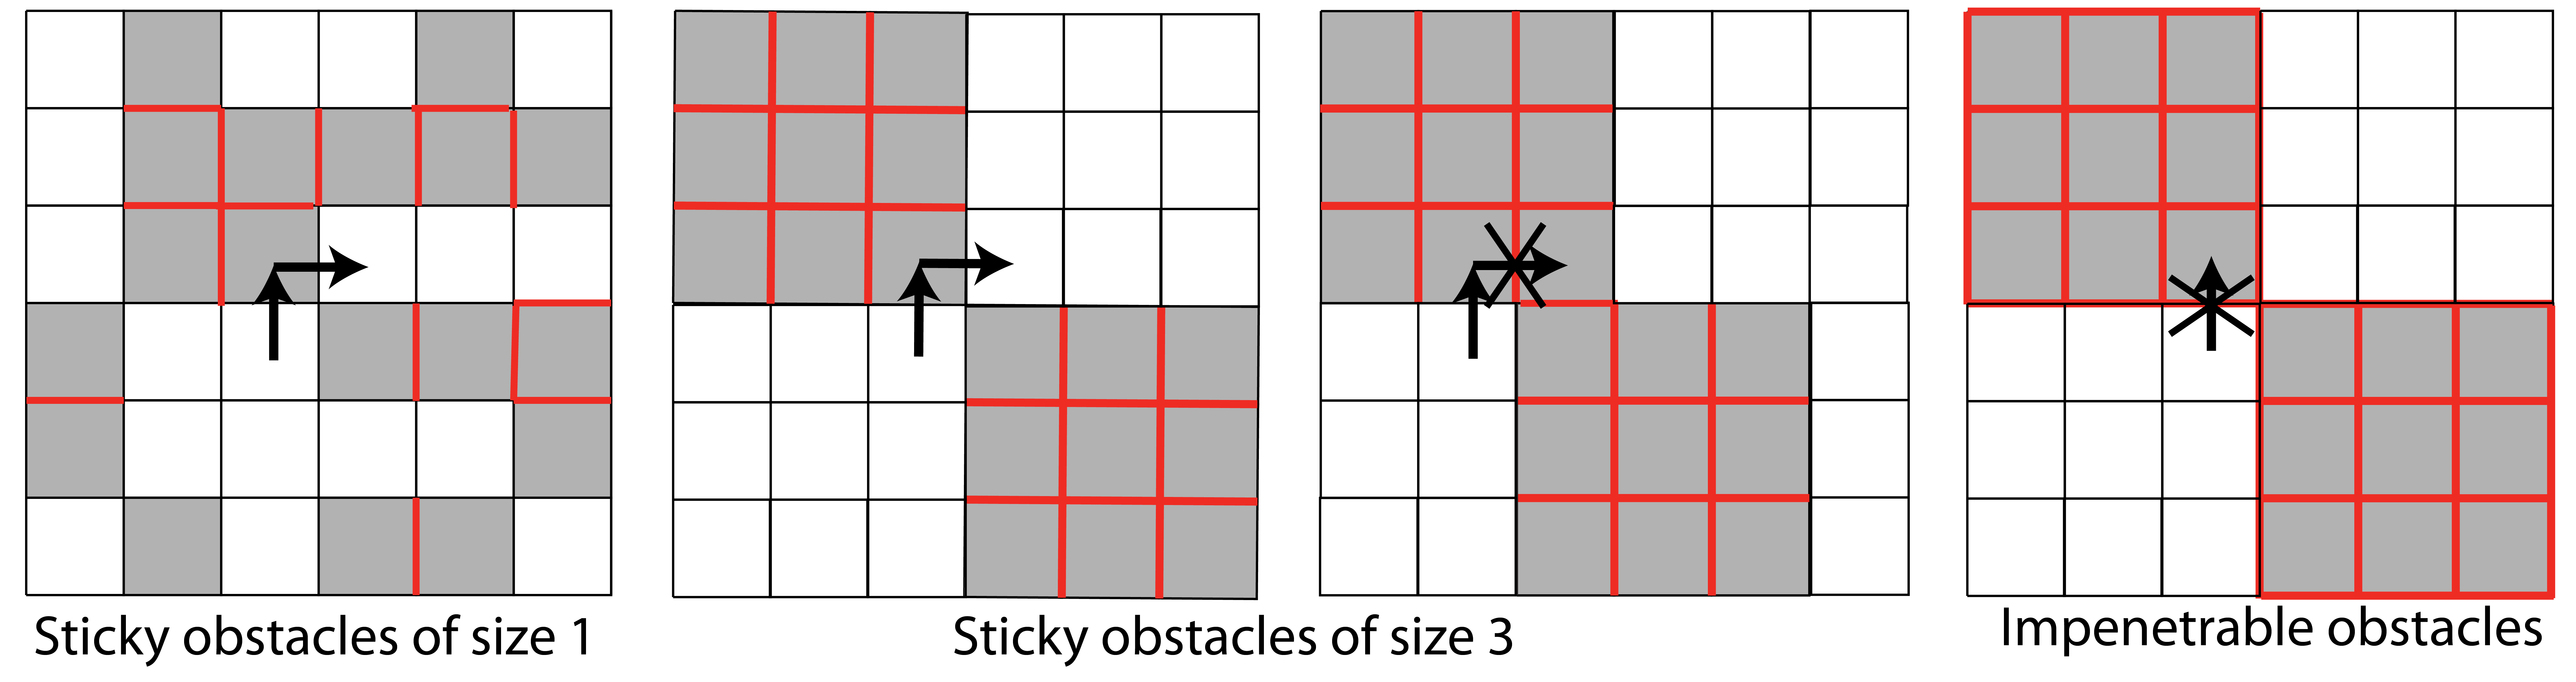
\includegraphics[width=150mm]{figs/ch02_soft/soft_size_moves.png}
  \end{center}
	\caption[Size effects cartoon]
    {Cartoon showing size effects for sticky and impenetrable
    obstacles. Red lines indicate borders between obstacles that
    cannot be crossed by a tracer.}\label{fig:size_moves}
\end{figure}
% figure 11

\subsection{Sticky obstacles of varying size} First, we examined tracer dynamics
on sticky obstacles of variable size \figrefp{fig:size_sticky}.  Qualitatively,
large sticky obstacles have a soft surface (binding can occur on surface sites,
although hops along the surface are still blocked), but a hard core (interior
sites are inaccessible).  A significant change in dynamics occurs when $ l_{\rm
  obst}$ increases above 1. Any obstacle with $l_{\rm obst} > 1$ is
fundamentally different from $l_{\rm obst} = 1$, because larger obstacles are
guaranteed to contain sites with an adjacent obstacle site. Increasing $l_{\rm
  obst}$ prevents hopping across the interior of any one obstacle, which can
hinder tracer motion. The cages are thus more robust.  Tracers can still hop
across corners, unlike in the case of a purely repulsive interaction
\figrefp{fig:size_moves}.

% figure 12 %
\begin{figure}[!b]
  \begin{center}
	  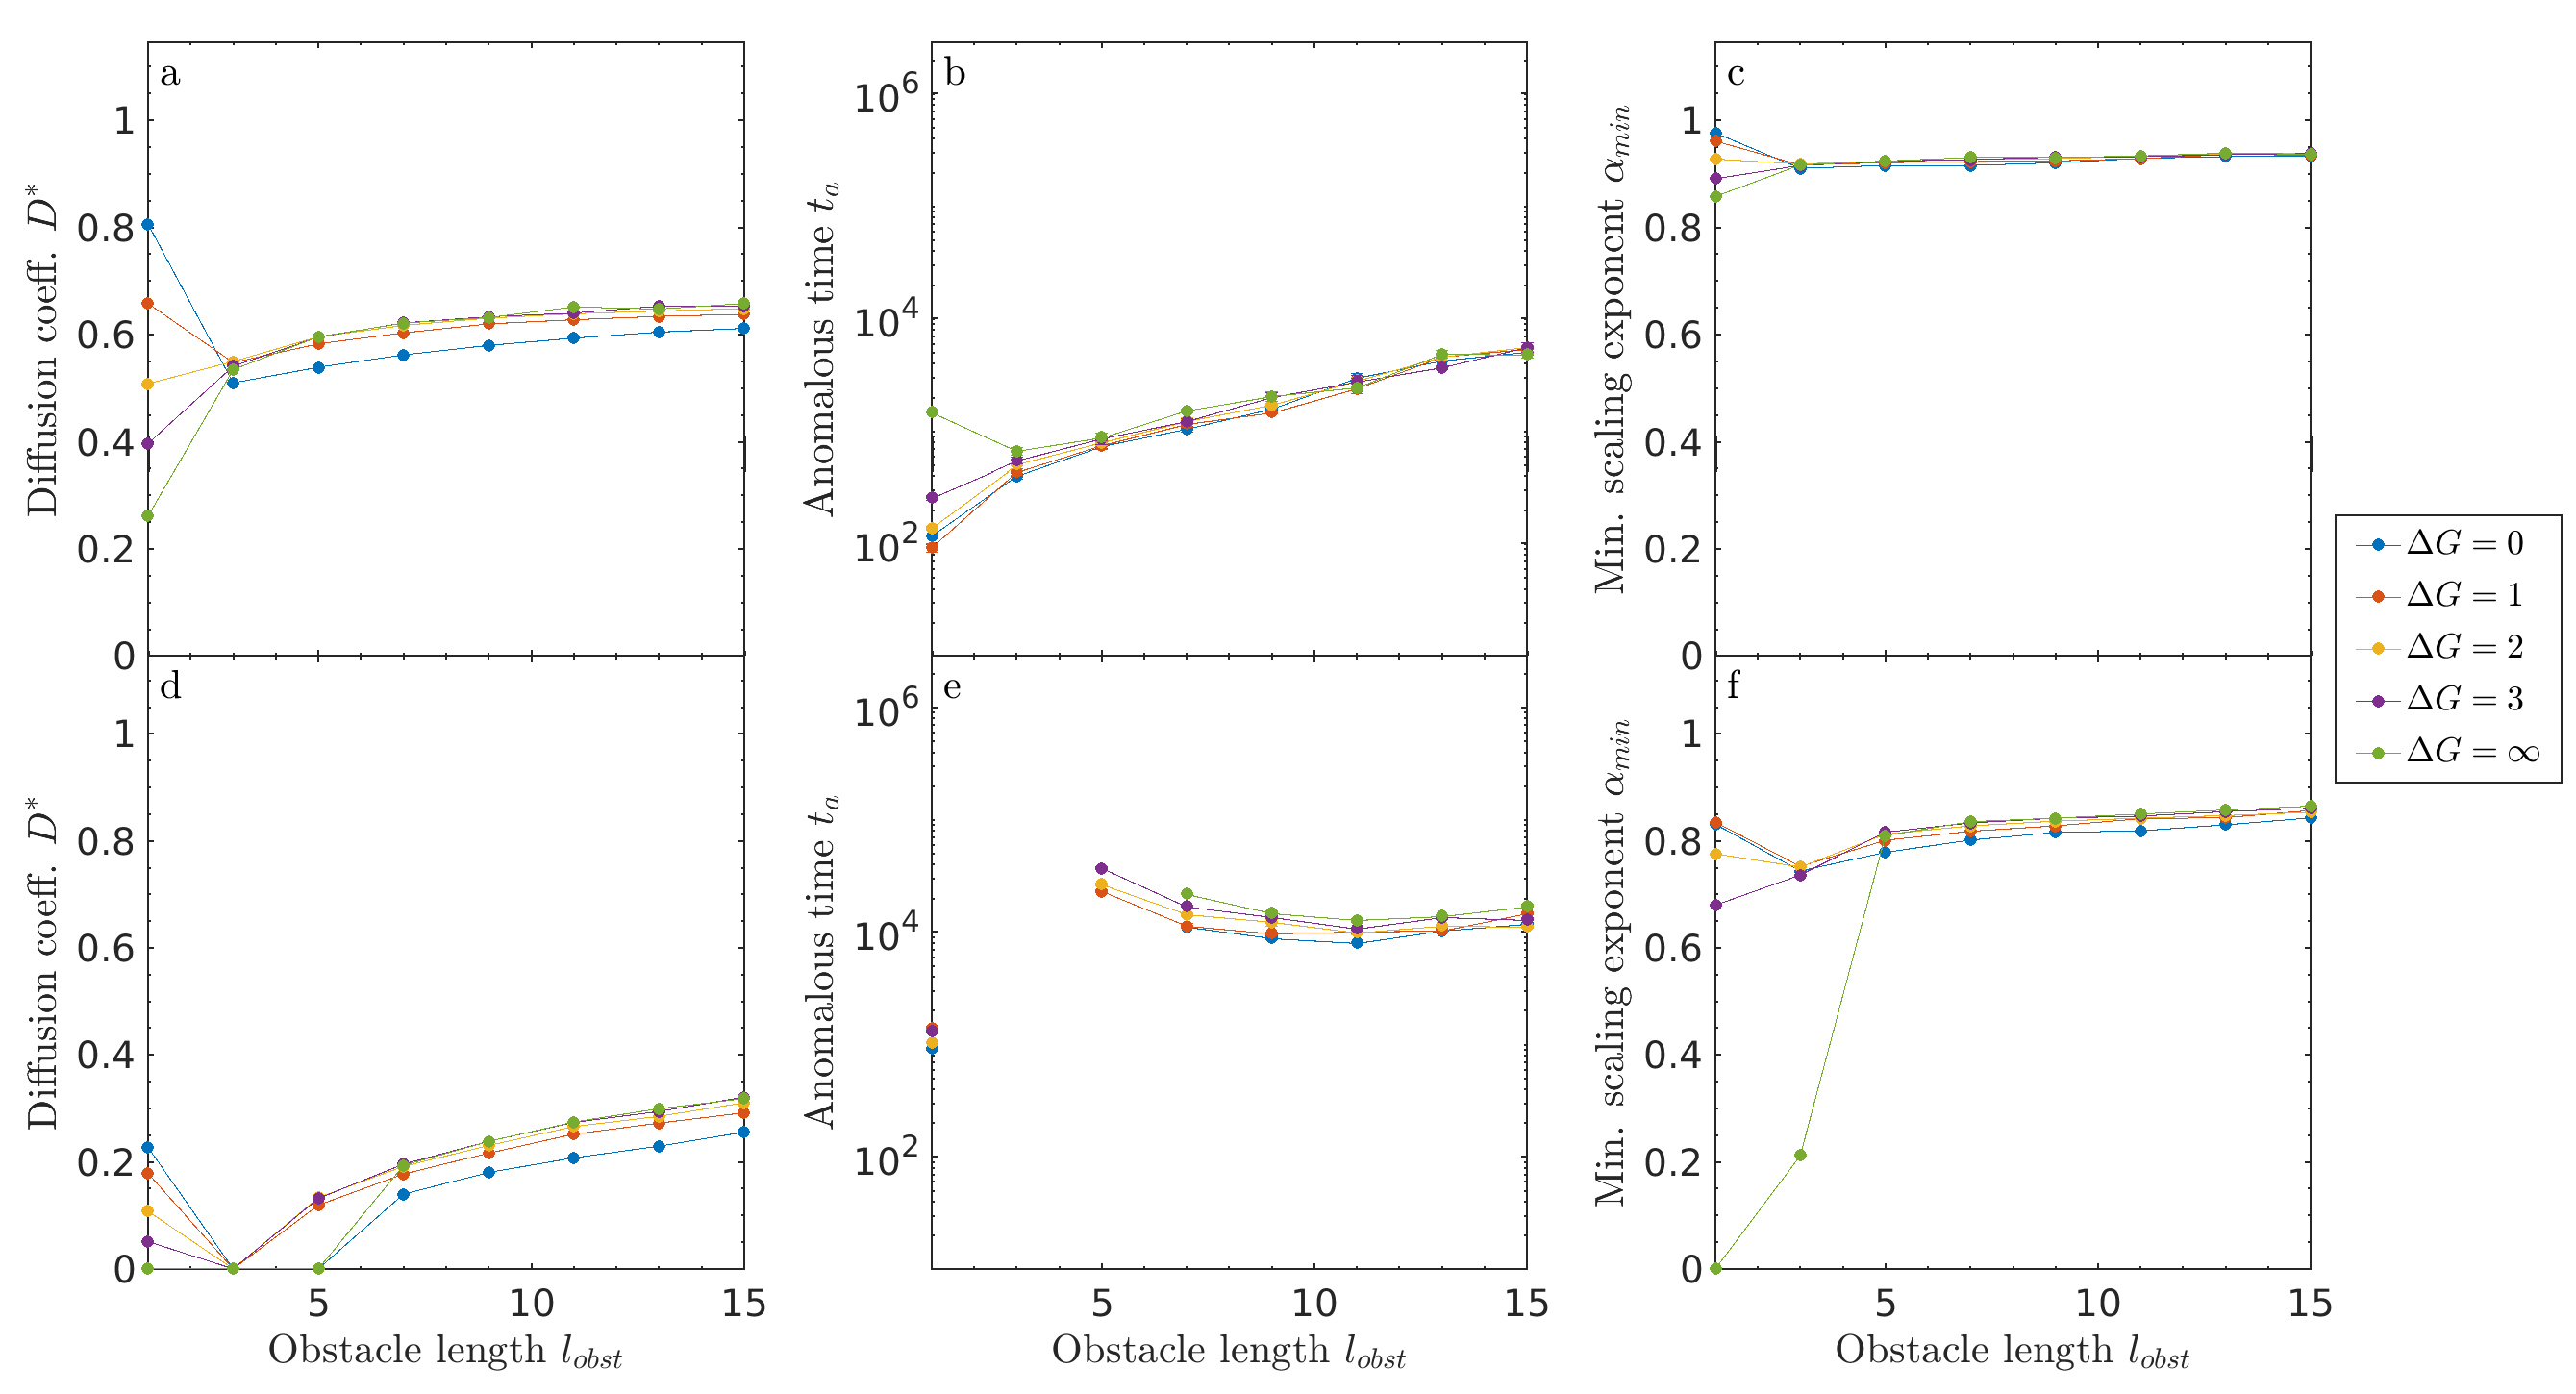
\includegraphics[width=150mm]{figs/ch02_soft/soft_size_sticky.png}
  \end{center}
	\caption[Sticky size effects]
    {Size effects for sticky obstacles in 2D.  (a, d) Diffusion
    coefficient $D^*$, (b, e) anomalous time $ t_a $, and (c, f)
    minimum scaling exponent $\alpha_{\min}$ as a function of
    obstacle filling fraction $\nu$ for $\nu=0.3$ (top) and $\nu =0.6$
    (lower).}\label{fig:size_sticky}
\end{figure}
% figure 12 %

The dependence of tracer dynamics on binding energy changes upon increasing the
obstacle size above 1 \figrefp{fig:size_sticky}.  For size-one obstacles,
particles can hop through a single obstacle, and so lower binding energy leads
to higher long-time diffusion coefficient. In contrast, with larger obstacles,
high binding energy leads to an increased diffusion coefficient. With higher
repulsion, a tracer is less likely to bind to the surface of an obstacle where
it can get stuck. Thus, for larger obstacles, higher repulsion can facilitate
motion.
 
For $l_{\rm obst}>3$, increasing obstacle size increases the cage size, and so
the long-term diffusion coefficient and the anomalous time both increase
smoothly, in agreement with previous work on impenetrable
obstacles~\cite{ellery_characterizing_14}.  The anomalous time increases with
$l_{\rm obst}$ above 3, because the effective cage size increases: tracers take
longer to explore a cage to escape.  For $l_{\rm obst}\geq 3$ and small filling
fraction, the size dependence is roughly energy independent.  The dynamics are
dominated by blocked $ \mathbf {obstacle} \rightarrow \mathbf {obstacle} $
moves, rather than by the energy dependence of $ \mathbf {empty} \rightarrow
\mathbf {obstacle} $ moves.  For low filling fraction, $\alpha_{\min}$ remains
$>0.9$, suggesting that obstacle caging effects are minimal.


Next, we examined a higher packing fraction $\nu = 0.6$, chosen because it is
between $\nu^l$ and $\nu^u$ for size-1 obstacles in 2D. The effects of obstacle
size on percolation are significant, leading to larger changes in behavior than
for $\nu=0.3$.  As $l_{\rm obst}$ increases, obstacles are on average spaced
farther apart, which increases $\nu^l$.

In contrast, the upper critical concentration is more complicated, because now
each obstacle contains within it obstacle-obstacle interfaces.  The upper
critical concentration decreases below $0.6$ for $l_{\rm obst} = 3$, and
therefore the dynamics are anomalous at all times; $t_a$ diverges and $D^*$ goes
to zero.  Above $l_{\rm obst} = 3$, the upper critical concentration increases
with increasing obstacle size.  For $l_{\rm obst} = 5$, $\nu^u>0.6$, leading to
long-time Fickian diffusion.  Here, $t_a$ decreases with $l_{\rm obst}$, because
the time required for a tracer to escape a cage is not dominated by the cage
size (as it was for low $\nu$), but by the time needed to find a gap between
cages.  As $l_{\rm obst}$ increases, the gaps become larger on average, lowering
the escape time.  Overall, above $l_{\rm obst} = 5$, the behavior is only mildly
dependent on either obstacle size or binding energy, making the long-time
diffusivity primarily a function of the filling fraction.

% figure 13 %
\begin{figure}[!hb]
  \begin{center}
	  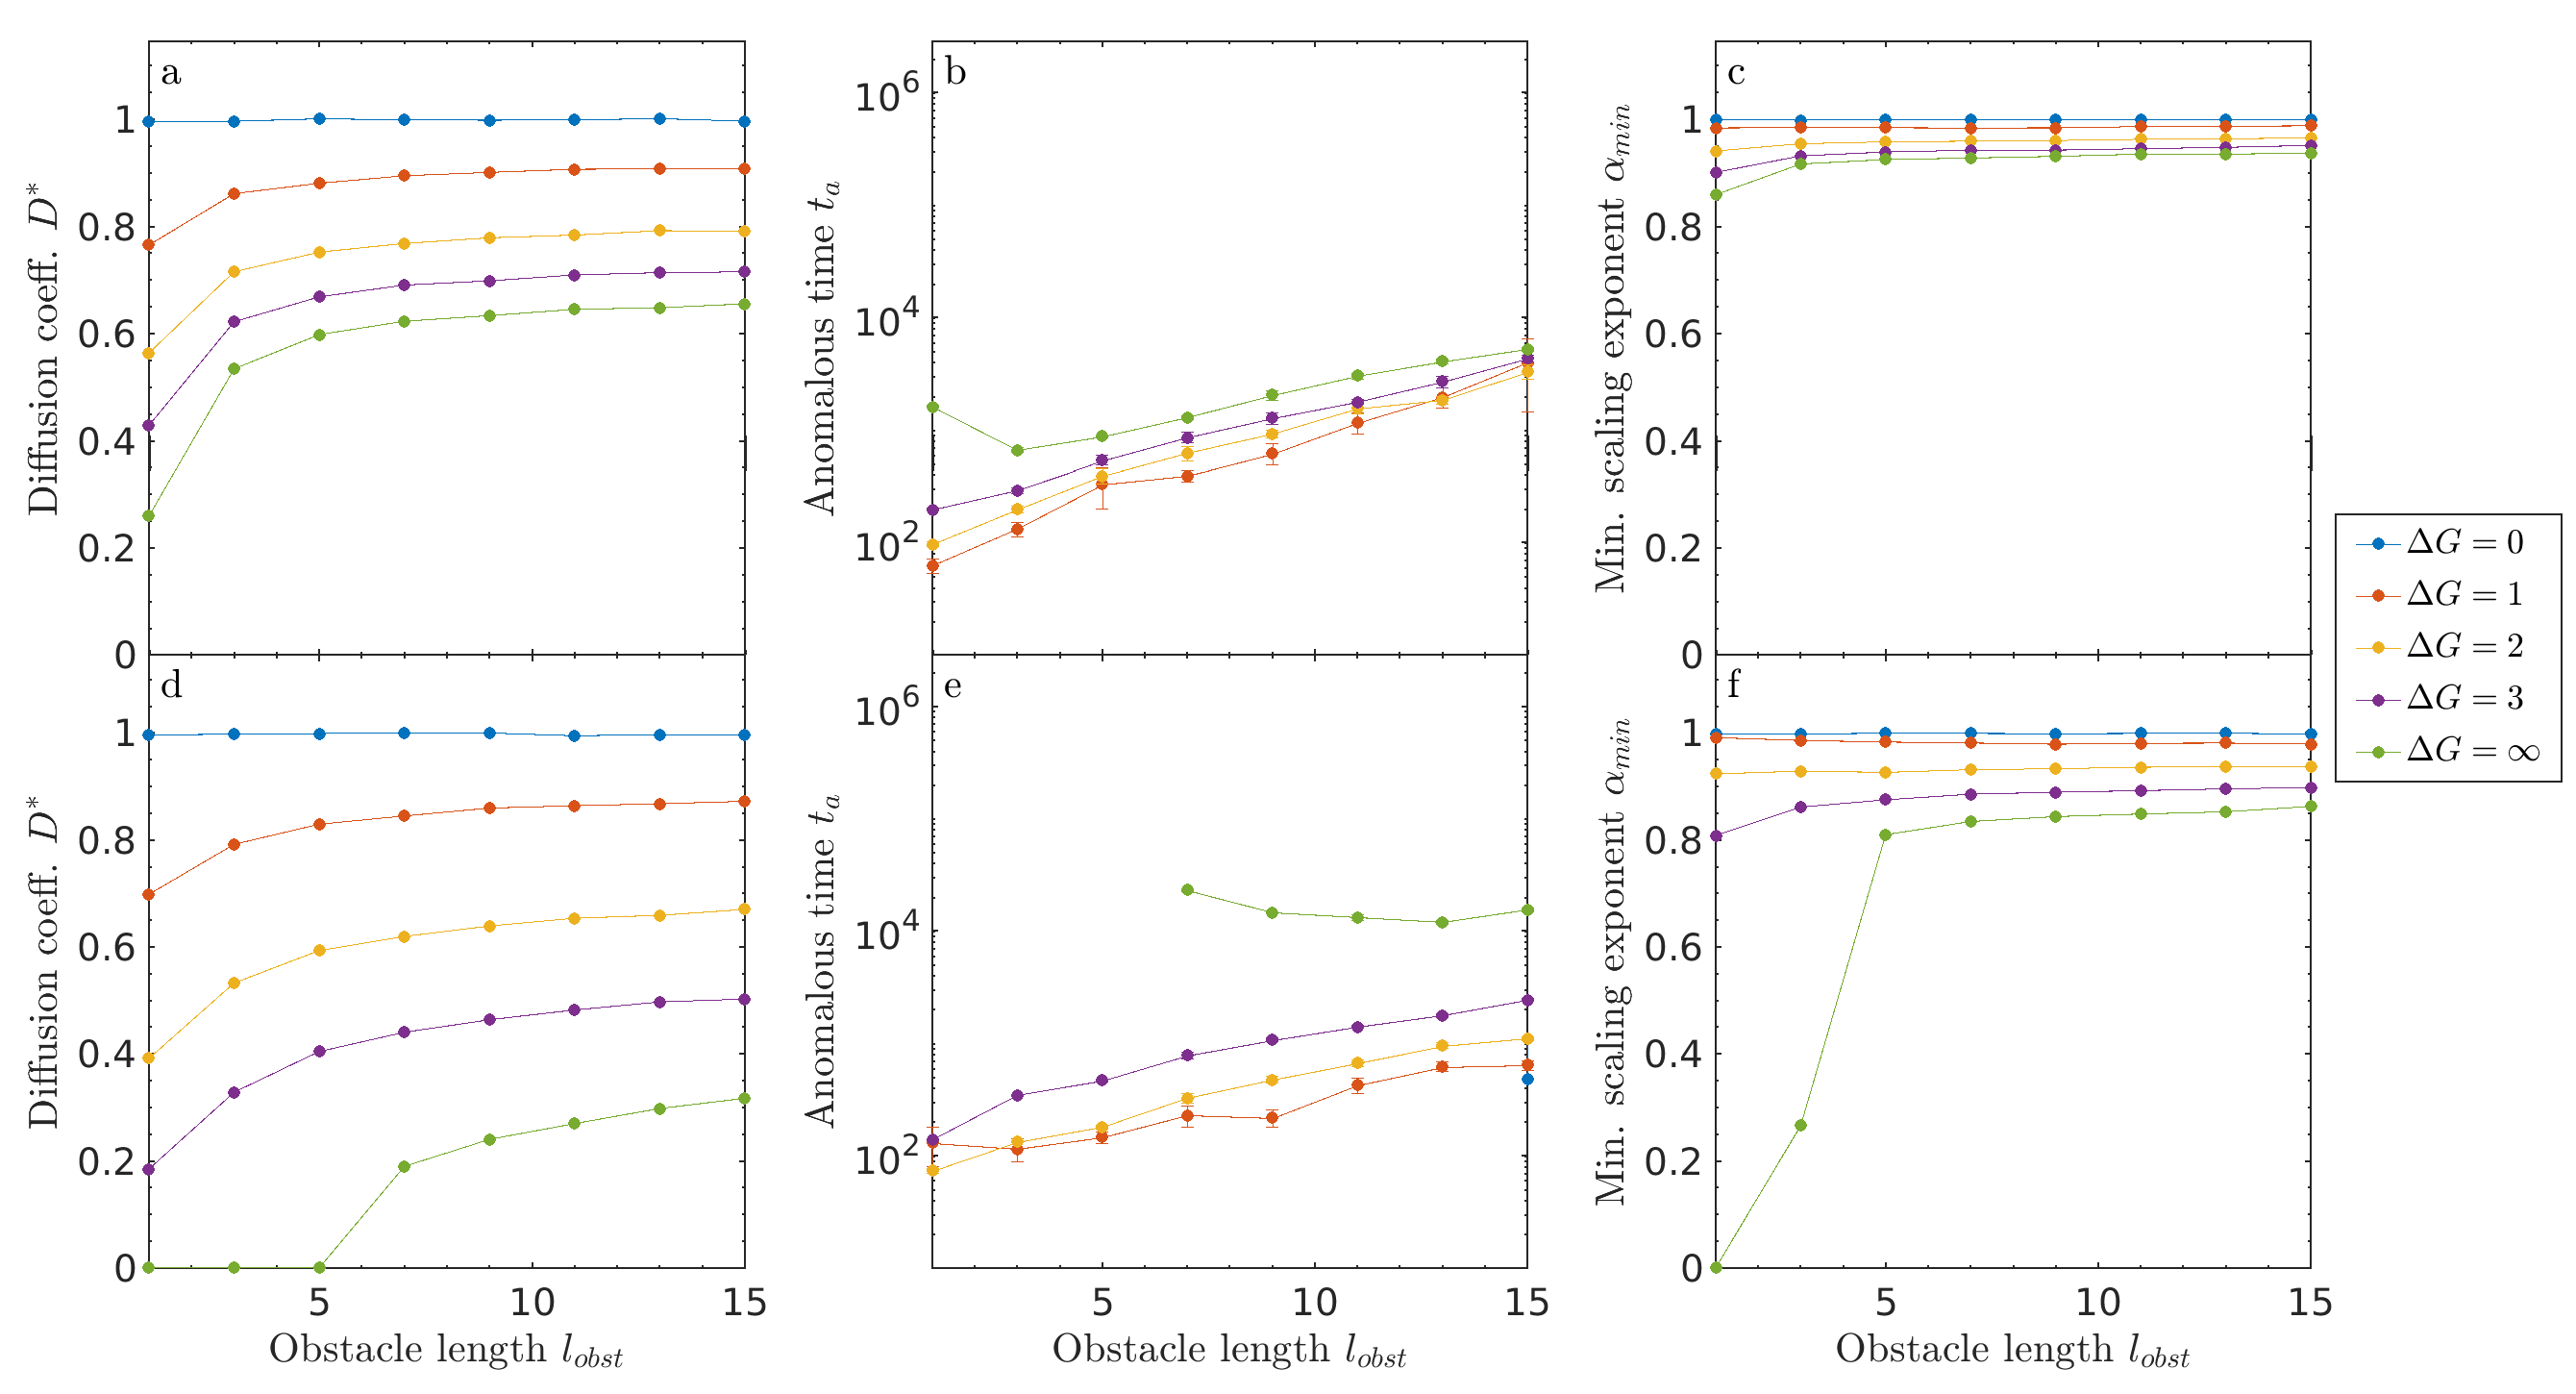
\includegraphics[width=150mm]{figs/ch02_soft/soft_size_slippery.png}
  \end{center}
	\caption[Slippery size effects]
    {Size effects for slippery obstacles in 2D.  (a, d)
    Diffusion coefficient $D^*$, (b, e) anomalous time $ t_a $, and
    (c, f) minimum scaling exponent $\alpha_{\min}$ as a function
    of obstacle filling fraction $\nu$ for $\nu=0.3$ (top) and
    $\nu =0.6$ (lower).}\label{fig:size_slippery}
\end{figure}
% figure 13 %

\subsection{Slippery obstacles of varying size}

Understanding the effects of variable obstacle size on tracer motion is more
straightforward for the case of slippery obstacles, because the difference
between edge and interior obstacle sites is eliminated
\figrefp{fig:size_slippery}. In the perfectly slippery limit, increasing $l_{\rm
  obst}$ effectively lowers the number of binding sites: tracers experience the
binding energy change only when binding to obstacle edge sites, but can move
freely through obstacle interior sites. Therefore, $D^*$ and $\alpha_{\min}$
increase with obstacle size, an effect that is larger for higher filling
fraction, because obstacle overlaps at high filling fraction lower the fraction
of obstacles that impede motion and cage tracers. In nearly all cases, $t_a$
increases with obstacle size, because the effective cage size grows. The
exception occurs for impenetrable obstacles, where increasing $l_{\rm obst}$
increases the size of vacancies between cages, allowing caged tracers to escape
more quickly.

\section{Conclusion}

In this chapter, we have studied a lattice model of tracer particles that
diffuse and experience crowding due to immobile obstacles. While most previous
work has considered hard (impenetrable) obstacles, we consider soft (penetrable)
obstacles characterized by a binding free energy that allows tracers to overlap
with obstacles. We also consider the effects of varying the tracer mobility
while bound, including the limiting cases of `sticky' obstacles (which
immobilize bound tracers) and `slippery' obstacles (which allow full tracer
mobility), as well as the intermediate regime between the two.

In some cases, diffusion in crowded media leads to dynamics that are anomalous
($r^2 \sim t^\alpha$) with a constant $\alpha$~\cite{hofling_anomalous_13}.
However, our system typically does not give a power law dependence of the MSD on
time delay; this has been seen by others~\cite{ellery_modeling_16,
  jeon_protein_16}.  As a result, we quantified a long-time diffusion constant
($D^*$), the timescale on which the systems transitions from anomalous to
Fickian ($t_a$), and the minimum instantaneous anomalous exponent
($\alpha_{\min}$).

Our results demonstrate the key differences between sticky and slippery
obstacles.  For sticky obstacles, increasing the obstacle filling fraction
decreases the diffusion coefficient and increases the degree of anomalous
diffusion. Above an upper critical occupancy $ \nu^u \approx 0.72 $ in 2D,
diffusion becomes anomalous at all times, independent of binding energy.  In the
sticky case, the minimum anomalous exponent $ \alpha_{\min} $ monotonically
decreases with filling fraction, because adding obstacles creates more cages in
which tracers become transiently confined.

For slippery obstacles, by contrast, tracers always reach normal diffusion after
a sufficiently long time; even increasing the filling fraction above the
percolation threshold does not eliminate tracer motion. For nonzero binding free
energy, we find a novel non-monotonic dependence of $D^*$ on filling fraction:
increasing the filling fraction away from zero introduces binding sites that
slow tracer diffusion, but for sufficiently high filling fraction, bound
mobility allows tracer motion along clusters of obstacles.  The anomalous
exponent decreases with binding energy magnitude, but varies non-monotonically
with filling fraction. For low filling fraction, $\alpha_{\min}$ decreases as
more obstacles are added, because binding transiently traps tracers on isolated
obstacles. For sufficiently high density, diffusion becomes more normal when
tracers hop along clusters of obstacles while bound.  For intermediate
`semi-slippery' obstacles, we demonstrate that in the crossover from sticky to
slippery behavior: $D^*$, $\alpha_{\min}$, and $t_a$ vary smoothly. Increasing
bound diffusion always makes the diffusion coefficient larger and the diffusive
motion less anomalous.

We varied obstacle size to examine how relatively large obstacle domains affect
tracer motion in our model. For sticky obstacles, increasing obstacle size above
1 led to a sharp jump in tracer properties. This occurs because larger obstacles
always contain interior obstacle sites, which are inaccessible to tracers in the
sticky model.  For large obstacles, increasing repulsive binding energy tends to
increase the tracer diffusion coefficient, because tracers spend less time
trapped in a binding site.
 
For slippery obstacles, perimeter and interior obstacle sites are both
accessible, which means that varying obstacle size has effects that are easier
to understand intuitively. The diffusion coefficient and anomalous exponent
increase with obstacle size, because larger obstacles lead to a fewer
obstacle-empty boundaries.  The effect of obstacle size on $t_a$ varied with
filling fraction, due to competing effects on increasing cage size and
increasing gaps between cages.

Our models separately represent effects of soft interactions (through the
binding energy) and bound-state motion (through obstacle
stickiness/slipperiness).  Sticky and slippery obstacles show dramatically
different tracer dynamics, even at short time and low filling fraction. Slippery
obstacles lead to a diffusion coefficient which varies non-monotonically with
filling fraction, with high values at both high and low obstacle density.  As
the filling fraction increases from zero, tracers are more and more inhibited by
obstacles.  However, as the obstacle density increases, particles which bind can
more easily move between obstacles.  This may describe transport factor motion
within the nuclear pore complex, where transport factors can slide on the
disordered FG Nup~\cite{raveh_slideandexchange_16}.  Therefore, biological
systems may use soft interactions and slippery obstacles to allow particle
diffusion, even in the highly crowded cellular interior.

Our work highlights how soft interactions\ and bound-state mobility can
dramatically change tracer motion. These effects are relevant to biological
systems, ranging from membraneless organelles to lipid rafts.  Although most
previous theoretical work on crowded diffusion has focused on the anomalous
exponent, these biological examples highlight the importance of changes in the
diffusion coefficient. For example, proteins which do not passage through the
nuclear pore complex on biologically relevant time scales (minutes to hours)
cannot have biological effects, and so the speed of passage is the fundamentally
important biological quantity. The long-time diffusion coefficient varies
dramatically in our model between hard obstacles, sticky soft obstacles, and
slippery soft obstacles \figrefp{fig:compare}.  Thus, the effective permeability
of obstacles and the degree to which bound particles can diffuse can be used by
cells to tune macromolecular motion.
